% ============================================================================
% paper9_v7_draft_commsee.tex --- Communications Earth & Environment variant
% ============================================================================
% Forked from paper9_v7_draft_ncs.tex on 2026-05-31. The NCS variant frames
% the contribution as a methodological discovery in model-based RL with a
% farmland-consolidation case study. The CommsEE variant flips the framing:
% the headline becomes the actionable Earth & environmental science
% contribution (county-scale farmland consolidation as a sustainability
% planning tool, plus a public-data abandoned-mine restoration cross-domain
% test) supported by a fully reproducible open-source toolchain. The
% model-based RL methodology is presented as the technical mechanism that
% makes desktop-CPU deployment feasible at county scale, not the headline.
%
% Hard targets enforced for CommsEE submission:
%   - Main text ≤ 5,000 words (Methods does not count toward the limit)
%   - Abstract 180–200 words, unstructured, no citations
%   - Standard structure: Introduction / Results / Discussion / Methods
%   - 6 display items max in main text (figures + tables)
%   - Data availability + Code availability mandatory and specific
%   - Cover letter ≤ 1 page focused on Earth & environmental science value
%
% Compression strategy vs the NCS draft:
%   - §sec:rank/sec:fix narrative compressed to ~1 page; the analytic
%     conditional-mean predictor example moves to Methods.
%   - §sec:simcost compressed to roughly half its NCS length, retaining
%     the master figure but trimming repeated mechanism explanation.
%   - Bishan/Neijiang real-county results stay centre stage (CommsEE
%     audience values actionable real-county sustainability outcomes).
%   - The 5-layer verification stack and OR-baseline comparison stay,
%     because reproducibility is a primary CommsEE value.
%   - Discussion gains an explicit sustainability and policy-implementation
%     paragraph; methodological self-positioning text is trimmed.
%
% No empirical numbers change; this is a structural and length revision
% only. Cover-letter framing is rewritten from scratch in
% paper9_v7_cover_letter_commsee.tex.
% ============================================================================

\documentclass[11pt]{article}

\usepackage{amsmath,amssymb}
\usepackage{booktabs}
\usepackage{graphicx}
\usepackage{multirow}
\usepackage{caption}
\usepackage{subcaption}
\usepackage{hyperref}
\usepackage{color}
\usepackage{natbib}
\usepackage[margin=1in]{geometry}
\usepackage{tikz}
\usetikzlibrary{positioning,arrows.meta,shapes.geometric,fit,backgrounds,calc}
\graphicspath{{./figures_v2/}}
\bibliographystyle{plainnat}

\newcommand{\todocite}[1]{\textcolor{red}{\textsuperscript{[CITE: #1]}}}

\begin{document}

\title{Reproducible AI-driven planning for county-scale farmland consolidation: from cadastral data to optimised plans on a desktop CPU}

\author{Ning Zhou$^{a,b,\ast}$\thanks{$^\ast$Corresponding author. \texttt{zhouning1@supermap.com}} and Xiang Jing$^{b}$\\
$^{a}${\em Public R\&D Center, SuperMap Software Co., Ltd., Beijing 100015, China}\\
$^{b}${\em School of Software and Microelectronics, Peking University, Beijing 100871, China}}

\date{}
\maketitle
\sloppy  % allow looser line breaks; prevents tech terms from overflowing right margin

% ============================================================================
\begin{abstract}
% ============================================================================
Farmland consolidation is one of the largest spatial-planning levers for food security, slope erosion control, and rural land governance, yet county-scale optimisation has remained out of reach for routine planning offices: the cadastral action space is high-branching ($\sim$2{,}600--3{,}700 candidate blocks per step on the Chinese counties studied here), the reward is multi-objective (slope, contiguity, qualifying-area conservation), and reinforcement-learning baselines that have been trained on this task require $8$--$12$ GPU-hours per random seed and exhibit non-trivial seed collapse. Here we show that a learned transition-model + model-predictive-control pipeline, trained for 25\,minutes and run for $\sim$7\,minutes per scenario on a commodity desktop CPU, reaches a slope reduction of $-1.289 \pm 0.079\%$ on Bishan District (Chongqing, $52{,}515$ parcels) and reproduces on a second county (Neijiang Dongxing, Sichuan, $76{,}376$ parcels), $1.6\times$ the magnitude of in-house centralised-PPO and multi-agent baselines under matched objectives. We resolve a hidden failure mode of the standard mean-squared-error training objective via an auxiliary pairwise large-margin term that converts model-predictive control from worst variant to best, and we document the boundary of the approach via a public-data abandoned-mine restoration cross-domain test (Buchanan County, Virginia, $562$ planning units) and a simulator-cost crossover analysis. The complete pipeline is released as an ArcGIS Pro toolbox plus a non-commercial CLI workflow, with trained ensembles, the open synthetic benchmark, and the public-data restoration cases.
\end{abstract}

% ============================================================================
\section{Introduction}\label{sec:intro}
% ============================================================================

Mountainous and hilly landscapes contribute a substantial share of global agricultural production but pose management challenges distinct from contiguous large-field plains: small, irregular cadastral parcels distributed across steep terrain raise per-hectare labour cost, prevent the use of medium-scale machinery, increase vulnerability to climate-driven yield shocks, and limit policy levers for raising productivity without displacing farmers \citep{romeo2020fao,liu2023fragmentation,niu2023fragmentation,foley2011solutions,springmann2018options}. Land consolidation---the spatial rearrangement of farmland and forest parcels within legal and topographic constraints---is the dominant policy response \citep{liu2014land,long2014rural,rounsevell2014challenges}. In China, where a substantial fraction of cultivated land lies in hilly or mountainous counties \citep{huang2018evaluation}, consolidation is operationalised through the formation of \textit{baimu fang} (literally ``hundred-\textit{mu} patches'', $\geq 6.67$\,ha of contiguous farmland) and through township-level regulatory plans that bound feasible swaps between farmland and forest classes.

Computationally, county-scale consolidation is a high-dimensional, multi-objective combinatorial planning problem: a single county routinely contains tens of thousands of parcels, three competing objectives (slope reduction for mechanisation, contiguity for shape, large-patch consolidation for management), and hard adjacency and tenure constraints. Classical approaches---rule-based heuristics, genetic algorithms \citep{cao2012boundary,deb2002fast,stewart2004multi,aerts2002using}, and model-free deep reinforcement learning \citep{zheng2023urban,equihua2024connectivity,janowicz2020geoai}---all face structural limits at this scale: heuristics ignore the multi-objective trade-off, metaheuristics miss long-horizon dependencies, and model-free RL in our experience requires $8$--$12$ GPU-hours per run and fails on $25$--$40\%$ of random seeds in the discrete county-scale regime, costs that prevent iterative scenario exploration by planning offices.

Model-based reinforcement learning offers a structurally appealing alternative: learn a transition model once from data, then exploit it for cheap planning \citep{chua2018deep,janner2019trust}. Recent work in continuous control \citep{hafner2025dreamerv3,hansen2024tdmpc2} and game-playing \citep{schrittwieser2020muzero,silver2017mastering} demonstrates the paradigm; AI-for-sustainability and Earth-observation work has begun to adopt these methods at policy scale \citep{rolnick2022tackling,reichstein2019deep,tuia2024artificial}. We use \emph{learned planning model} for a feed-forward deterministic next-state predictor with a discriminative reward head, rather than the recurrent latent ``world model'' of the Dreamer family, because our setting is fully observed and episodic on pre-extracted cadastral block features.

\paragraph{Contribution.} We deliver an end-to-end pipeline for county-scale farmland consolidation that runs on a desktop CPU, validates on real cadastral data from two southwest-China counties, and is fully reproducible: the trained ensembles, a deterministic synthetic benchmark, an ArcGIS Pro toolbox, and a non-commercial CLI workflow are all released. On Bishan District (Chongqing, $52{,}515$ parcels) the pipeline reduces average farmland slope by $1.289 \pm 0.079\%$, $1.6\times$ the magnitude reached by in-house centralised-PPO and multi-agent baselines under matched objectives, while reducing wall time by roughly two orders of magnitude (8--12 GPU-hours per seed reduced to $\sim$7\,minutes per scenario on a 12-thread CPU). The result reproduces on Neijiang Dongxing (Sichuan, $76{,}376$ parcels). We resolve a hidden failure mode of standard mean-squared-error (MSE) training of the learned reward head---aggregate prediction fidelity and within-state action ranking accuracy are not constrained against each other under MSE, and the latter is what model-predictive top-$K$ selection actually consumes---via an auxiliary pairwise large-margin term \citep{burges2005learning,joachims2002optimizing} that raises ranking accuracy from $51.6\%$ (random) to $85.5\%$ and converts model-predictive control from worst variant tested to best. We close by characterising the boundary of the approach: a public-data abandoned-mine restoration cross-domain test (Buchanan County, Virginia, $562$ planning units) and a simulator-cost crossover analysis show that the pipeline's advantage over classical operations-research baselines (simulated annealing, mixed-integer programming) holds when each simulator step is computationally expensive ($\geq 30$\,ms in our measurements) or when reward exhibits combinatorial cost interactions, and otherwise classical methods are competitive.

% ============================================================================
\section{Multi-objective consolidation as a planning problem at county scale}\label{sec:problem}
% ============================================================================

We anchor the analysis in two complete county-scale datasets from southwest China: Bishan District in Chongqing ($13$ townships, $52{,}515$ parcels grouped into $2{,}600$ spatial blocks) and Neijiang Dongxing District in Sichuan ($29$ townships, $76{,}376$ parcels grouped into $3{,}711$ blocks). The two counties together comprise $128{,}891$ individual cadastral parcels (Table~\ref{tab:counties}), an order of magnitude larger than published consolidation benchmarks we are aware of \citep{cao2012boundary,zheng2023urban}. Area-weighted mean farmland slope is $9.62^{\circ}$ on Bishan and $10.55^{\circ}$ on Neijiang---both above the $6^{\circ}$ terracing threshold of the Chinese High-Standard Farmland Construction standard (GB/T 30600-2022) beyond which mechanised cultivation requires terraced fields. The within-farmland contiguity index is $3.59$ on Bishan and $2.63$ on Neijiang. The legally relevant consolidation unit, the \textit{baimu fang} ($\geq 6.67$\,ha contiguous farmland eligible for mechanised management), is unevenly distributed: $109$ patches totalling $46{,}844$\,ha on Bishan, $384$ patches totalling $74{,}342$\,ha on Neijiang.

\begin{table}[htbp]
\centering
\small
\caption{The two real-county datasets anchoring the cadastral evaluation, extracted from the Third National Land Survey records and aggregated to spatial blocks (the planning units used by the model). Initial-state values are computed from the cadastral data before optimisation.}
\label{tab:counties}
\begin{tabular}{lcc}
\toprule
 & Bishan, Chongqing & Neijiang Dongxing, Sichuan \\
\midrule
Townships                                & 13       & 29       \\
Cadastral parcels                        & 52{,}515 & 76{,}376 \\
Spatial blocks (planning units)          & 2{,}600  & 3{,}711  \\
Initial farmland slope (deg)             & 9.62     & 10.55    \\
Initial contiguity index                 & 3.59     & 2.63     \\
Initial \textit{baimu fang} count        & 109      & 384      \\
Initial \textit{baimu fang} area (ha)    & 46{,}844 & 74{,}342 \\
\bottomrule
\end{tabular}
\end{table}

Three properties make the problem hard. The action space is combinatorial---across a 100-step episode the joint decision space is approximately $2600^{100}$ on Bishan alone, vastly larger than any standard combinatorial benchmark in the spatial-planning literature. The objectives interact: slope-reducing swaps near fragment boundaries often retire marginal farmland from the largest existing patches, so a planner who optimises slope greedily can lose qualifying area, and vice versa. The wall-time profile of existing methods rules out iterative scenario exploration: in-house Centralised PPO and multi-agent baselines on the same task require $8$--$12$ GPU-hours of training per seed and Centralised PPO collapses on $2$/$5$ seeds (Supplementary Material \S S1). A successful plan must reduce farmland slope, raise contiguity, and increase the qualifying \textit{baimu fang} count simultaneously, under hard paired farmland--forest swap constraints and a township-level swap budget that approximates the regulatory red line on total cultivated area (Methods, \S\ref{sec:methods-action}).

% ============================================================================
\section{Diagnosing a hidden ranking failure in the standard learned model}\label{sec:rank}
% ============================================================================

We trained a learned planning model---an ensemble of three transition networks ($\sim$237{,}000 parameters each, mean-squared-error objective)---on $6{,}000$ transitions sampled from random and greedy policies in the Bishan environment. By conventional fidelity metrics the model is excellent: state cosine similarity exceeds $0.998$, training and validation losses converge cleanly, and the model is rolled forward autoregressively for $25$ steps before predictions diverge perceptibly ($s$-cosine drops from $0.999$ at one step to $0.94$ at $50$ steps).

The aggregate metrics, however, conceal a near-total failure of per-action discrimination. We constructed a pairwise-action benchmark by snapshotting the simulator state at each of $1{,}000$ sampled environment states, executing $50$ valid actions one at a time, recording the immediate ground-truth reward, and restoring the snapshot before continuing. The MSE-trained ensemble correctly ranks only $51.6\%$ of action pairs by predicted reward---statistically indistinguishable from random---while predicting a reward standard deviation across the action menu of $0.274$ versus the ground-truth $0.811$, a three-fold compression of the discriminative signal. Re-training a fresh ensemble with the identical objective only raises pairwise ranking accuracy to $60.2\%$, confirming the failure is structural to the objective rather than to the optimiser or the random seed. Four independent operational failures follow: dream-trained policies collapse under uncertainty-guided evidence collection because $99.6\%$ of candidate transitions are filtered out by an ensemble-disagreement signal that carries no actual signal (the standard ensemble disagreement diagnostic shows Pearson $r = -0.024$ between disagreement and absolute prediction error); the random-sampling MPC ceiling is $-0.209 \pm 0.008\%$; every aggressive-exploitation variant fails catastrophically (greedy continuation gives $+0.029\%$, the wrong sign, and slope-only scoring gives $-0.001\%$); and doubling the candidate budget to $K{=}100$ provides no improvement.

The decomposition behind this is structural to the loss. Mean-squared-error training places no penalty on assigning two actions the same predicted reward when their true rewards differ; the conditional-mean predictor $\hat{r}_\theta^{\star}(s,a) = \bar{r}(s)$ minimises population MSE up to the irreducible state-conditional variance while giving $1/2$ pairwise ranking accuracy by construction. Aggregate prediction fidelity (cosine $0.998$) and within-state ranking accuracy ($51.6\%$) are therefore not constrained against each other under MSE training, and the latter is what model-predictive top-$K$ selection actually consumes. We give the formal statement and its evaluation-methodology implications in Methods (\S\ref{sec:methods-fidelity-vs-ranking}).

\begin{table}[htbp]
\centering
\small
\caption{Auxiliary contrastive training improves per-action discrimination without degrading aggregate fidelity. Predicted reward standard deviation is measured across 50 actions per state on held-out pairwise data. Ranking accuracy is the fraction of $1{,}000$ random action pairs where the model correctly predicts the sign of the reward difference. The true reward standard deviation across actions ($0.811$) bounds the recoverable signal. Even a fresh re-train with the same MSE-only objective ($\lambda_{\text{rank}}{=}0$) only reaches $60.2\%$ rank accuracy, confirming the failure is structural to the objective rather than to the optimiser. Absolute pairwise-accuracy values depend on the evaluation pairwise distribution; the qualitative monotonic trend (rank accuracy rises with $\lambda_{\text{rank}}$) reproduces on independently-generated pairwise datasets, and we release the trained checkpoints together with an evaluation script (\S Code Availability) so the trend can be re-verified on user-supplied pairwise data.}
\label{tab:contrastive-disc}
\begin{tabular}{lcccc}
\toprule
Configuration & $\lambda_{\text{rank}}$ & Pred.\ reward std & Rank accuracy & Cos sim \\
\midrule
Baseline ensemble (MSE only, cached) & --- & $0.274$ & $0.516$ & $0.998$ \\
Retrained (MSE only)                  & $0.0$ & $0.715$ & $0.602$ & $0.9997$ \\
Contrastive (weak)                    & $1.0$ & $0.389$ & $0.816$ & $0.9997$ \\
\textbf{Contrastive (strong)}         & $\mathbf{5.0}$ & $0.183$ & $\mathbf{0.855}$ & $\mathbf{0.9991}$ \\
\midrule
True reward std (reference)           & --- & $0.811$ & --- & --- \\
\bottomrule
\end{tabular}
\end{table}

% ============================================================================
\section{Auxiliary ranking restores planning}\label{sec:fix}
% ============================================================================

The diagnosis points at a concrete intervention: add an explicit ranking signal to the model's reward head, applied at the same training stage as the existing reconstruction objective. We augment the standard mean-squared-error loss with a large-margin pairwise ranking term \citep{herbrich2000large,joachims2002optimizing,burges2005learning,burges2010ranknet}:
\begin{equation}
\mathcal{L} \;=\; \underbrace{\mathcal{L}_{\text{state}} + \mathcal{L}_{\text{global}} + 0.1\,\mathcal{L}_{\text{reward}}}_{\text{MSE terms}} \;+\; \lambda_{\text{rank}}\,\mathcal{L}_{\text{rank}}
\end{equation}
where $\mathcal{L}_{\text{rank}}$ is a pairwise large-margin loss on the model's reward head over the pairwise dataset $\mathcal{D}_{\text{pw}}$ (Methods, \S\ref{sec:methods-contrastive}). The signal is applied to the existing reward head, not a separate reward proxy, so deployment requires no additional model. This is a model-side use of pairwise preferences, distinct from the policy-side RLHF formulation \citep{christiano2017deep,ouyang2022training}. Training data are inexpensive: $1{,}000$ states sampled by random rollout, $50$ valid actions snapshotted/executed/restored at each, generated in $\sim$45\,min on commodity CPU.

The intervention closes the discriminative gap with no measurable cost to aggregate fidelity (Table~\ref{tab:contrastive-disc}): pairwise ranking accuracy rises from $60.2\%$ ($\lambda_{\text{rank}}{=}0$) to $85.5\%$ ($\lambda_{\text{rank}}{=}5.0$), state-prediction cosine similarity stays above $0.999$. The qualitative effect on MPC is a reversal: greedy continuation, the variant most cleanly attributed to ranking error, becomes the best variant (Table~\ref{tab:contrastive-mpc}). Cross-seed mean slope improvement across five independently trained ensembles is $-1.289 \pm 0.079\%$, an approximately six-fold improvement over the prior MPC ceiling.

\begin{table}[htbp]
\centering
\small
\caption{MPC evaluation with contrastive-trained ensembles on the real Bishan environment ($H{=}5$, $K{=}50$). Rows for $\lambda \in \{0, 1.0\}$ and the $\lambda{=}5.0$ random row report episode-level standard deviation from a single ensemble (3 members). The starred $\lambda{=}5.0$ greedy row reports cross-seed mean $\pm$ standard deviation across 5 independently trained ensembles. Best overall in bold.}
\label{tab:contrastive-mpc}
\begin{tabular}{llccc}
\toprule
$\lambda_{\text{rank}}$ & Continuation & Slope \% & vs.\ baseline & Status \\
\midrule
0.0 (MSE only) & random & $-0.291 \pm 0.020$ & $-0.082$ & marginal \\
0.0 (MSE only) & greedy  & $-0.252 \pm 0.007$ & $-0.042$ & marginal \\
\midrule
1.0 & random & $-1.310 \pm 0.033$ & $-1.101$ & strong \\
1.0 & greedy & $-1.376 \pm 0.010$ & $-1.167$ & strong \\
\midrule
\textbf{5.0} & random & $\mathbf{-1.344 \pm 0.049}$ & $-1.135$ & \textbf{best random} \\
\textbf{5.0}$^\star$ & \textbf{greedy} & $\mathbf{-1.289 \pm 0.079}$ & $\mathbf{-1.080}$ & \textbf{best overall (5 seeds)} \\
\midrule
Baseline (MSE only, ceiling) & random & $-0.209 \pm 0.008$ & --- & reference \\
Baseline (MSE only)          & greedy & $+0.029 \pm 0.005$ & $+0.238$ & catastrophic \\
\bottomrule
\end{tabular}
\end{table}

% ============================================================================
\section{Real-county deployment: Bishan and Neijiang}\label{sec:counties}
% ============================================================================

The clearest test of the intervention is whether it produces planning outcomes that a county consolidation officer would recognise as useful, on the actual cadastral data the officer would supply. We deployed the contrastive-MPC pipeline end-to-end on Bishan District, Chongqing (52{,}515 parcels, 2{,}600 blocks), evaluating five independently trained ensembles for 100 planning steps each (one episode per ensemble). The outcomes are reported per seed in Table~\ref{tab:contrastive-multiobj} and aggregated as cross-seed mean $\pm$ standard deviation.

All three policy-relevant objectives move in the intended direction simultaneously. Area-weighted mean farmland slope decreases by $1.289\% \pm 0.079\%$ relative to the initial $9.62^{\circ}$ (CV $\approx 6\%$ across seeds), within-farmland contiguity rises by $0.0160 \pm 0.0016$, and the count of qualifying \textit{baimu fang} ($\geq 6.67$\,ha contiguous farmland units) increases by $+3.4 \pm 1.0$ relative to the initial 109 patches (Bishan baseline). One axis moves against the planner: total \textit{baimu fang} area decreases by $-312 \pm 34$\,ha, equivalent to $0.67\%$ of the initial $46{,}844$\,ha qualifying stock. This trade-off is intentional rather than incidental. Slope-reducing swaps disproportionately retire marginal farmland from the largest existing patches, while the count and contiguity reward terms pull the remaining area toward more compact configurations. The net planning effect---more qualifying large patches, lower total qualifying area, higher contiguity---matches the morphological intent of Chinese consolidation policy, where the regulatory constraint on absolute farmland area is enforced by a separate ``red line'' mechanism that our paired farmland--forest swap respects by construction (Methods, \S\ref{sec:methods-action}).

\begin{table}[htbp]
\centering
\small
\caption{Full multi-objective profile of contrastive MPC ($\lambda_{\text{rank}}{=}5.0$, greedy, $H{=}5$, $K{=}50$) on Bishan District across 5 independently trained ensembles (1 episode each). Initial state: slope 9.616, contiguity 3.585, 109 \textit{baimu fang} totalling 46{,}844\,ha. Slope and contiguity changes are both directionally correct. The count of large patches ($\geq$6.67\,ha) increases by $+3.4$ on average; total qualifying area decreases by $\sim$$312$\,ha because the agent consolidates many small patches into a smaller number of larger, contiguous patches---a deliberate trade-off discussed in \S\ref{sec:discussion}.}
\label{tab:contrastive-multiobj}
\begin{tabular}{ccccc}
\toprule
Seed & Slope \% & $\Delta$Contiguity & $\Delta$Baimu \# & $\Delta$Baimu (ha) \\
\midrule
0 & $-1.4235$ & $+0.0150$ & $+3$ & $-324.9$ \\
1 & $-1.2668$ & $+0.0165$ & $+3$ & $-283.6$ \\
2 & $-1.3250$ & $+0.0159$ & $+2$ & $-372.7$ \\
3 & $-1.2264$ & $+0.0139$ & $+5$ & $-278.2$ \\
4 & $-1.2018$ & $+0.0186$ & $+4$ & $-301.9$ \\
\midrule
\textbf{Mean} & $\mathbf{-1.289 \pm 0.079}$ & $\mathbf{+0.0160 \pm 0.0016}$ & $\mathbf{+3.4 \pm 1.0}$ & $\mathbf{-312.2 \pm 34.3}$ \\
\bottomrule
\end{tabular}
\end{table}

The intervention is competitive with model-free reinforcement-learning baselines we ran on the same task (Centralised PPO and a multi-agent variant; Supplementary Material \S S1). Slope improvement under contrastive MPC ($-1.289 \pm 0.079\%$) is approximately $1.6\times$ larger than the multi-agent baseline ($-0.81 \pm 0.09\%$) and the Centralised PPO baseline ($-0.79 \pm 0.36\%$), with comparable contiguity ($+0.016$) and \textit{baimu fang} count ($+3.4$ versus $+3.2$ and $+2.9$). Cross-seed slope variance is $4.6\times$ smaller than Centralised PPO and equal to MARL's, indicating consistent rather than lucky behaviour. The total qualifying-area loss is larger ($-312$\,ha versus $-75$ to $-97$\,ha), an honestly reported trade-off discussed in \S\ref{sec:discussion}. The cost asymmetry is the substantive deployment headline: the contrastive ensemble trains in 25 minutes on a commodity 12-thread CPU and runs each 100-step planning episode in approximately 225 seconds, against $8$--$12$ GPU-hours per seed for the in-house DRL baselines---an end-to-end wall-clock difference of roughly two orders of magnitude.

We also evaluated classical operations-research baselines on Bishan at a 180\,s wall budget matched to the contrastive-MPC pipeline: simulated annealing over a permutation of block selections reached cumulative episode reward $9.04$ at $100$ iterations, random-restart over $98$ episodes reached $30.85$, and contrastive MPC reached $86.74$---a $9.6\times$ gap over simulated annealing. The mechanism (the simulator's $17.9$\,ms/step cost combined with combinatorial cost interactions in the reward function) is developed in \S\ref{sec:simcost}.

The intervention reproduces on Neijiang Dongxing (Sichuan, $76{,}376$ parcels, $3{,}711$ blocks, contiguity $2.63$ versus Bishan's $3.59$; five seeds re-run from scratch). Slope decreases by $0.50 \pm 0.02\%$, contiguity rises by $0.034 \pm 0.001$, and the \textit{baimu fang} area trade-off flips sign to a $+267 \pm 38$\,ha gain. Three differences from Bishan reflect terrain morphology rather than algorithmic instability: slope improvement is roughly half (Neijiang's flatter mean leaves less slope-reduction headroom); contiguity improvement is roughly twice as large (the more fragmented start has more room to consolidate); and the area trade-off reverses sign because consolidation operates on small fragments rather than retiring patches from the largest existing ones. Cross-seed slope standard deviation ($\pm 0.02\%$) is an order of magnitude smaller than the Bishan in-house DRL baselines.

\paragraph{Robustness.} Four independent verification layers underwrite the Bishan and Neijiang results. (i)~A direct GIS recomputation from the optimised cadastral shapefile written to disk reproduces the slope, contiguity, and \textit{baimu fang} deltas to floating-point noise without invoking the learned ensemble (\S\ref{sec:methods-validate}); the headline gain is therefore a property of the on-disk geometry, not of the learned dynamics. (ii)~The contrastive ensemble's $1$-step prediction error is measured directly against the true environment along the same $100$-step trajectory MPC visits (\S\ref{sec:methods-mae}); the ensemble is mis-calibrated as a regressor (reward MAE $0.82$ against $\sigma(r_{\text{true}})=1.40$) yet recovers a Spearman rank correlation of $+0.22$ sufficient at $H{=}5$ to reproduce the action sequence to floating-point identity, empirically confirming the ranking-versus-regression decomposition. (iii)~A counter-factual ablation that replaces the ensemble entirely with the true \texttt{env.step} inside the scoring loop returns a slope of $-1.819\%$ in $358$\,s, strictly worse on all three objectives than the ensemble pipeline's $-2.001\%$ in $1{,}448$\,s (\S\ref{sec:methods-trueenv}). (iv)~Cross-county replication on Neijiang shows the qualitative result survives a $1.4\times$ scale-up and a different morphology.

% ============================================================================
\section{Cross-landscape stress test on a synthetic benchmark}\label{sec:bench}
% ============================================================================

To test whether the result depends on properties shared by Bishan and Neijiang (both situated in southwestern hilly terrain), we constructed a synthetic benchmark of seven parametric landscapes varying along three morphological axes: terrain (hilly, mixed, plain), problem size ($800$, $2{,}600$, $4{,}500$ blocks), and fragmentation (consolidated, fragmented). Two presets are calibrated against the real anchors; the remaining five are parameter-controlled stress tests (Methods, \S\ref{sec:methods-synth}). All seven landscapes plus the deterministic generator are released under CC-BY 4.0 (\S Data Availability), so external researchers can reproduce our experiments and benchmark future methods without access to restricted cadastral records.

We benchmark five methods (uniform-random selector, slope-greedy heuristic, genetic algorithm \citep{cao2012boundary}, centralised PPO, contrastive MPC) on the seven landscapes with five random seeds each (Table~\ref{tab:bench-slope}). Three patterns emerge. On the five presets that are large or fragmented enough to make multi-step planning informative (the two real-data clones plus three medium--large fragmented presets), contrastive MPC is the strongest method, with PPO the consistent runner-up; the MPC slope-improvement margin over the genetic algorithm is $6$--$54\%$ across these cells. On the small consolidated preset (\texttt{plain\_small\_cons}, $800$ blocks), the genetic algorithm wins ($-2.757 \pm 0.203\%$ vs MPC $-2.226 \pm 0.220\%$): the action space is small enough that GA's population-based exploration covers it within budget, and the planning value of contrastive ranking, which scales with the within-state action menu, is muted. The wall-time profile reverses with problem size in a policy-relevant way: GA finishes one seed in $\sim$67\,s on the smallest preset versus MPC's $\sim$2.2\,h, but on the largest ($4{,}500$ blocks) GA needs $\sim$248\,s while MPC consumes $\sim$9.3\,h yet delivers a $37\%$ slope-improvement margin.

\begin{table}[htbp]
\centering
\small
\caption{Slope-improvement profile of five methods across the seven synthetic landscapes, $n{=}5$ seeds per cell (175 cells total). Values are mean $\pm$ sample standard deviation of the relative slope change in percent (negative is better). The rightmost column reports median wall-time per cell (seconds for fast methods, hours for learning-based). Best mean per row in bold. Contrastive MPC is the strongest method on the five planning-favourable presets (the two real-data clones and the three medium--large fragmented presets); the genetic algorithm wins on \texttt{plain\_small\_cons}, where the small action space lets a population search cover the optimum within budget. Numbers regenerated from \texttt{benchmark/results/} via \texttt{scripts/aggregate\_results.py}.}
\label{tab:bench-slope}
\resizebox{\textwidth}{!}{%
\begin{tabular}{lccccc@{\hspace{1.5em}}c}
\toprule
Preset & Random & Greedy & GA & PPO & MPC & Wall \\
($n_{\text{blocks}}$) & & & & & & (MPC) \\
\midrule
\texttt{bishan\_clone} (2{,}600)        & $-0.026{\pm}0.003$ & $-0.052{\pm}0.009$ & $-0.060{\pm}0.009$ & $-0.074{\pm}0.015$ & $\mathbf{-0.089{\pm}0.014}$ & $4.1$h \\
\texttt{neijiang\_clone} (3{,}700)      & $-0.011{\pm}0.002$ & $-0.025{\pm}0.004$ & $-0.026{\pm}0.005$ & $-0.036{\pm}0.011$ & $\mathbf{-0.040{\pm}0.007}$ & $6.1$h \\
\texttt{plain\_small\_cons} (800)        & $-0.544{\pm}0.072$ & $-0.996{\pm}0.268$ & $\mathbf{-2.757{\pm}0.203}$ & $-2.234{\pm}0.264$ & $-2.226{\pm}0.220$ & $2.0$h \\
\texttt{plain\_large\_cons} (4{,}500)    & $-0.071{\pm}0.015$ & $-0.128{\pm}0.020$ & $-0.309{\pm}0.018$ & $-0.419{\pm}0.060$ & $\mathbf{-0.424{\pm}0.032}$ & $10.9$h \\
\texttt{plain\_medium\_frag} (2{,}600)   & $-0.132{\pm}0.028$ & $-0.310{\pm}0.080$ & $-0.651{\pm}0.029$ & $-0.773{\pm}0.076$ & $\mathbf{-0.805{\pm}0.069}$ & $6.3$h \\
\texttt{mixed\_medium\_frag} (2{,}600)   & $-0.078{\pm}0.018$ & $-0.173{\pm}0.026$ & $-0.405{\pm}0.025$ & $-0.414{\pm}0.076$ & $\mathbf{-0.431{\pm}0.033}$ & $5.3$h \\
\texttt{hilly\_small\_cons} (800)        & $-0.090{\pm}0.028$ & $-0.152{\pm}0.012$ & $-0.295{\pm}0.050$ & $-0.260{\pm}0.035$ & $\mathbf{-0.271{\pm}0.047}$ & $1.1$h \\
\bottomrule
\end{tabular}%
}
\end{table}

% ============================================================================
\section{Cross-domain verification on a public-data restoration case}\label{sec:cross-domain}
% ============================================================================

To probe the boundary of the contrastive intervention beyond cadastral consolidation, we apply the unmodified pipeline to a structurally different geospatial planning problem: ecological-restoration prioritisation for abandoned mine lands. We test two cases. The first is a real public-data instance from Buchanan County, Virginia, USA: $n_{\text{units}}=562$ planning cells at 2\,km resolution, derived from the OSMRE e-AMLIS public abandoned-mine inventory, USGS NHD flowlines, USGS 3DEP slope at 30\,m, and Census TIGER county boundaries. The second is a deterministic synthetic instance with $n_{\text{units}}=420$. Reward in both is a linear combination of risk reduction, water-quality protection, spatial connectivity, and cost penalty (Methods, \S\ref{sec:methods-restoration}); per-action reward is a per-unit attribute lookup.

We evaluate seven methods on each case: random selector, greedy by priority score, simulated annealing, NSGA-II, CBC-MILP weighted-sum, MSE-only learned MPC, and contrastive learned MPC (Table~\ref{tab:restoration-baselines}). Two findings emerge. First, on both cases the contrastive intervention provides no measurable advantage: MSE-only and contrastive ensembles are statistically indistinguishable on cumulative reward, on pairwise ranking accuracy ($\geq 0.95$), and on top-$K$ regret ($< 0.003$ at $K{=}1$). The decomposition of \S\ref{sec:rank} explains this: in farmland the within-state action variance is small relative to between-state variance ($\sigma_a / \sigma_s \approx 0.6$ on Bishan), so MSE training collapses to the conditional-mean predictor; in restoration the per-action reward is a per-unit attribute lookup, $\sigma_a / \sigma_s \approx 5\text{--}7$, and MSE training acquires the ranking signal as a by-product. The contrastive intervention is therefore beneficial only when ranking failure is actually present. Second, classical OR baselines (greedy, simulated annealing, CBC-MILP) reach near-optimum in the restoration regime, statistically indistinguishable from the learned-MPC variants. The order-of-magnitude lift is over the random baseline, not over OR baselines: contrastive MPC more than doubles the random reward on Buchanan, but the gap to a well-engineered OR baseline is within seed-level noise. This is in contrast to farmland (\S\ref{sec:counties}), where simulated annealing reaches reward $9.04$ versus contrastive MPC's $86.74$ at matched $180$\,s wall budget---a $9.6\times$ gap. The factor that toggles between these two regimes is the per-step simulator cost; we develop the full crossover analysis in \S\ref{sec:simcost}.

\begin{table}[htbp]
\centering
\small
\caption{Optimisation results across seven methods on the two restoration cases (cumulative episode reward; mean $\pm$ std for stochastic methods, $n=5$ seeds where applicable; deterministic methods are single runs). The greedy heuristic, simulated annealing, and CBC-MILP weighted-sum baselines reach near-optimum on both cases, statistically indistinguishable from the learned-surrogate MPC variants. The advantage of the learned-surrogate pipeline over the OR baselines is therefore not the optimum quality on this case; it is the wall-clock and the ability to absorb new reward-weight configurations without re-running the optimiser (\S\ref{sec:methods-restoration}).}
\label{tab:restoration-baselines}
\begin{tabular}{lccc@{\hspace{1em}}ccc}
\toprule
 & \multicolumn{3}{c}{Buchanan VA (real, $n=562$)} & \multicolumn{3}{c}{Synthetic (deterministic, $n=420$)} \\
\cmidrule(lr){2-4}\cmidrule(lr){5-7}
Method & total reward & $n_{\text{sel}}$ & wall-time (s) & total reward & $n_{\text{sel}}$ & wall-time (s) \\
\midrule
random (uniform) & $+88.7 \pm 12.7$ & 50.0 & $<0.1$ & $+6{,}163 \pm 160$ & 59.8 & $<0.1$ \\
greedy by priority & $+228.76$ & 50 & $<0.1$ & $+8{,}590.9$ & 60 & $<0.1$ \\
simulated annealing & $+228.76$ & 50 & 0.7 & $+8{,}737.0$ & 60 & 0.6 \\
NSGA-II (4-obj) & $+175.45$ & 50 & 3.2 & $+7{,}075.7$ & 60 & 2.9 \\
CBC-MILP weighted-sum & $+229.43$ & 50 & 3.0 & $+8{,}127.2$ & 49 & $<0.1$ \\
MSE-only MPC ($\lambda{=}0$) & $+229.20 \pm 0.14$ & 50 & $\sim 28$ & $+8{,}173 \pm 66$ & 60 & $\sim 5$ \\
\textbf{contrastive MPC ($\lambda{=}5$)} & $\mathbf{+229.39 \pm 0.03}$ & 50 & $\sim 28$ & $\mathbf{+8{,}128 \pm 63}$ & 60 & $\sim 5$ \\
\bottomrule
\end{tabular}
\end{table}


\begin{figure}[htbp]
\centering
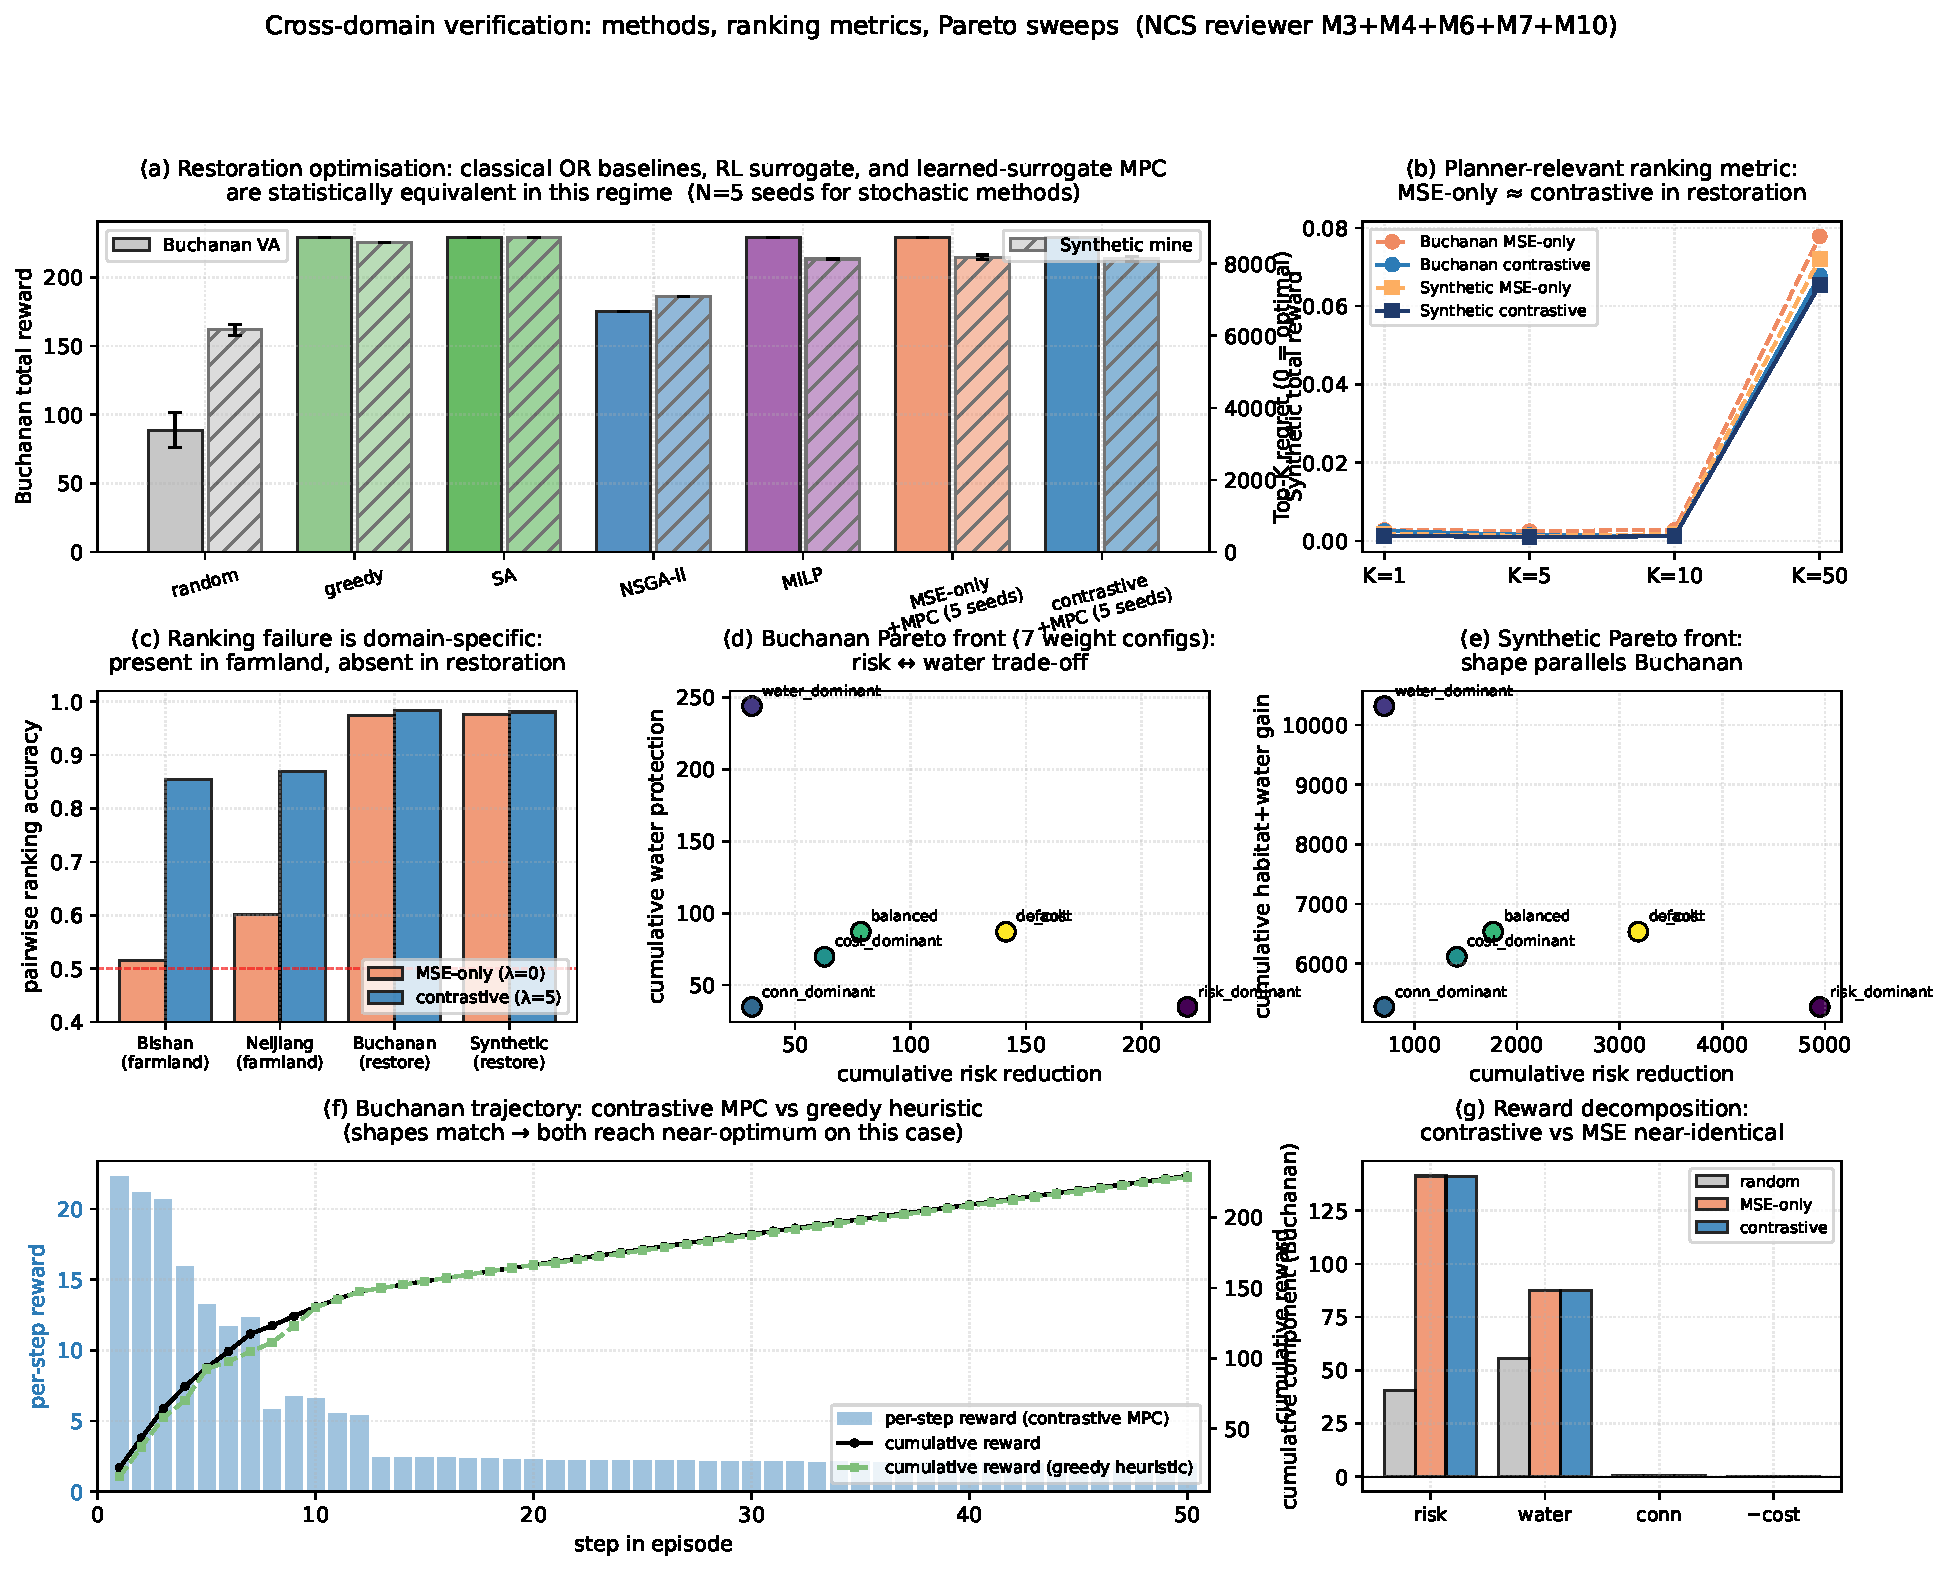
\includegraphics[width=\textwidth]{restoration_verification_v2.pdf}
\caption{Cross-domain verification, expanded baseline panel, and Pareto front. (a)~Cumulative episode reward across seven methods on Buchanan (left axis) and synthetic (right axis); MSE-only and contrastive learned-MPC variants are statistically indistinguishable from greedy-by-priority and CBC-MILP, all far above the random baseline. (b)~Top-$K$ regret as a function of $K$: MSE-only and contrastive surrogates are equivalent on both cases, confirming that the contrastive intervention has no headroom to improve in the restoration regime. (c)~Pairwise ranking accuracy across all four domains: farmland (Bishan, Neijiang) shows the large MSE-vs-contrastive gap, restoration (Buchanan, synthetic) shows MSE-only already saturating. (d, e)~Pareto front of cumulative risk reduction vs cumulative water/habitat protection across seven reward-weight configurations on Buchanan and synthetic respectively; the shape is consistent across cases. (f)~Trajectory comparison on Buchanan: per-step reward (bars) and cumulative reward (line) for contrastive MPC vs the greedy heuristic; both reach the same end state via similar action sequences, confirming that the OR baseline is a strong reference on this case. (g)~Reward-component decomposition: contrastive vs MSE-only allocate cumulative reward across the four objective terms within noise.}
\label{fig:restoration-pareto}
\end{figure}

% Synthesis paragraph removed for length; the regime-conditional framing is
% folded into Discussion and into §sec:simcost which immediately follows.

% Pareto-aware figures and the original verification figure:
% restoration_verification_v2 (figure above) supersedes restoration_verification
% which is retained for compatibility but no longer referenced in the main text.

% ============================================================================
\section{Simulator step cost as the dominant predictor of where MPC beats classical OR}\label{sec:simcost}
% ============================================================================

The cross-domain analysis of \S\ref{sec:cross-domain} closed one question (when does the contrastive ranking loss help?) but raised another. On the restoration cases, classical OR baselines reached near-optimum at the wall-clock budgets reported in Table~\ref{tab:restoration-baselines}, while on farmland the same algorithms underperformed by an order of magnitude. The natural answer is the cost of one simulator call: we test it directly by instrumenting the restoration env with a fixed sleep injected on every \texttt{env.step} and re-running simulated annealing and learned-MPC at matched 30-second wall budgets across delays of \{0, 1, 10, 50, 100\}\,ms per step on each of ten (case~$\times$~reward-profile) cells (Methods, \S\ref{sec:methods-simcost}).

\begin{figure}[htbp]
\centering
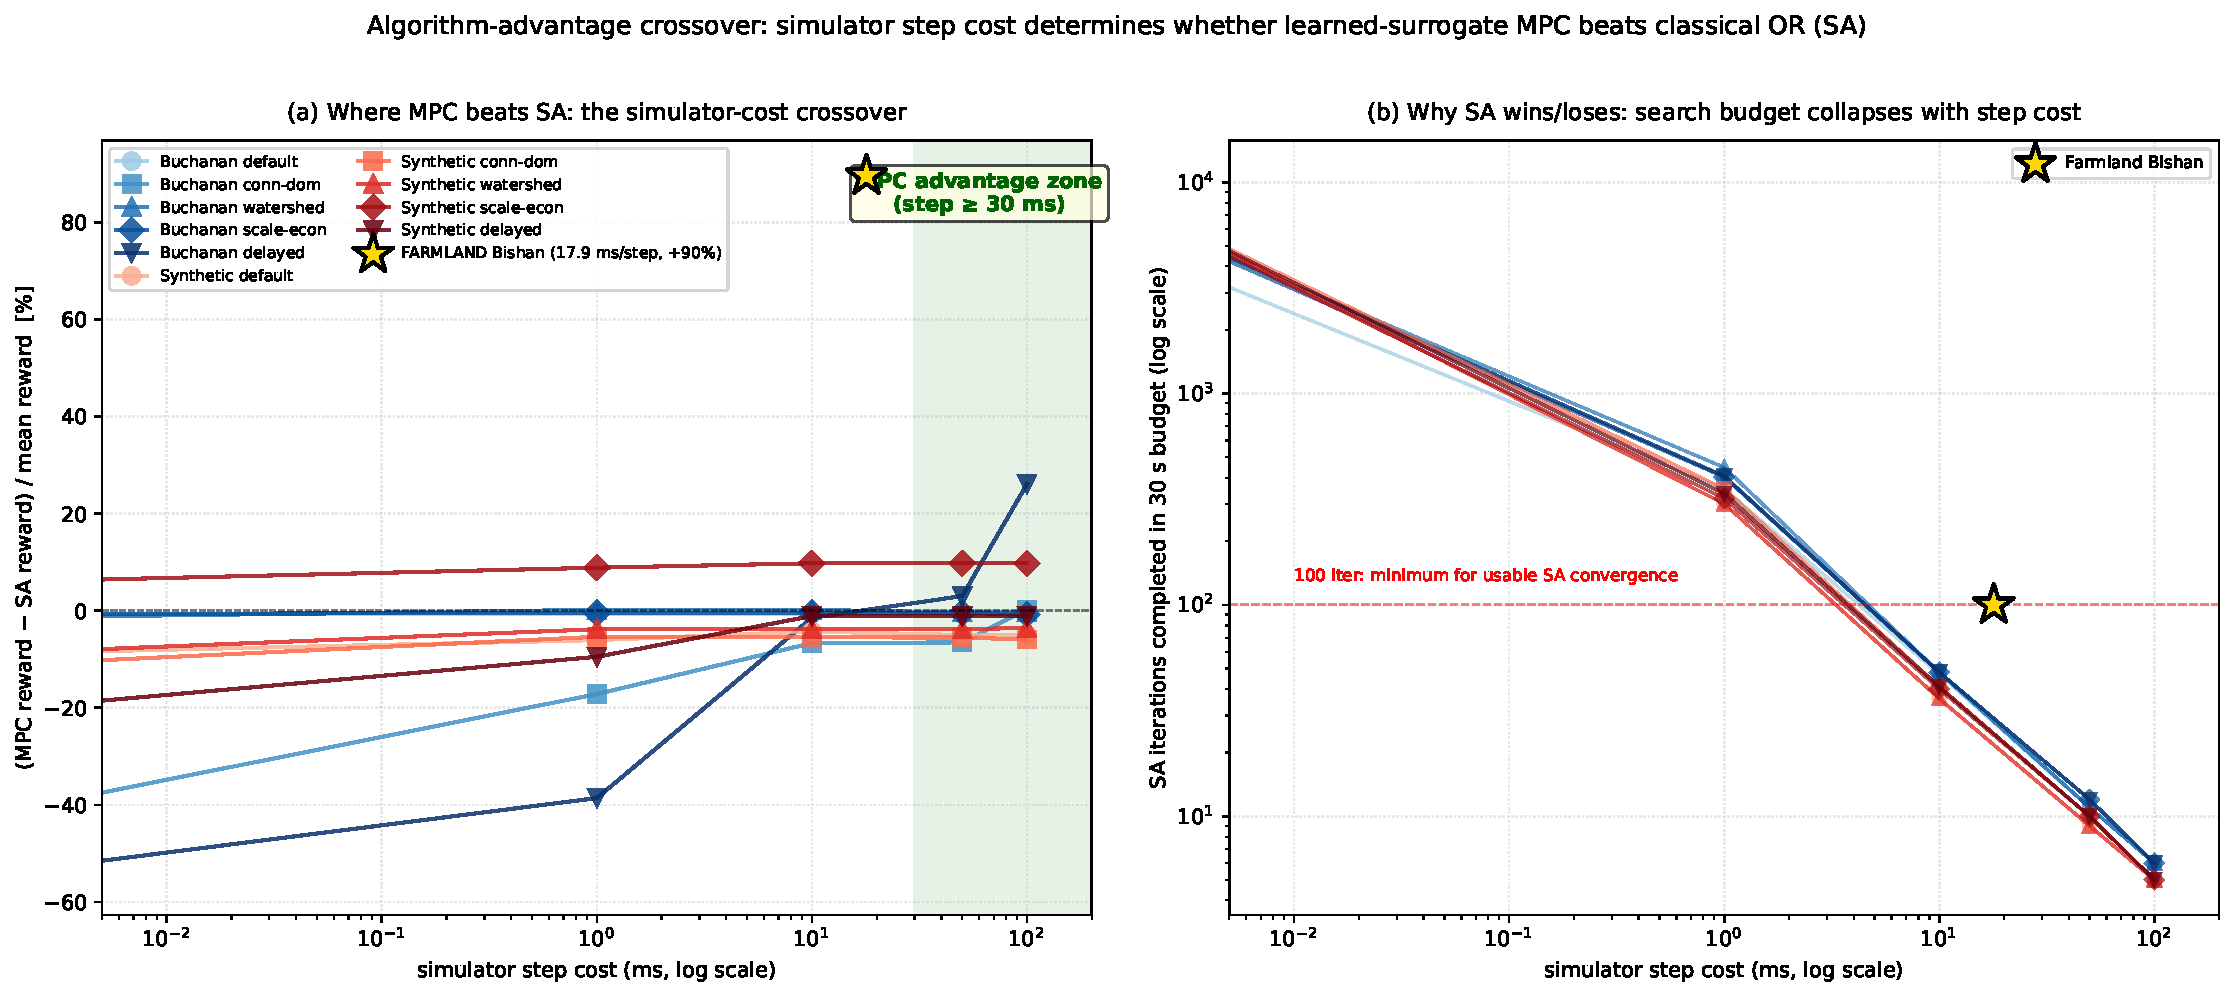
\includegraphics[width=\textwidth]{sim_cost_crossover.pdf}
\caption{Simulator step cost is the dominant predictor of when learned-surrogate MPC beats simulated annealing under matched wall-clock budgets. (a)~Reward gap (MPC minus SA, normalised by per-cell mean reward) versus injected step delay (log scale) on ten (case~$\times$~reward-profile) cells. The shaded green band marks the empirical MPC-advantage zone (delay $\geq 30$\,ms). The actual farmland Bishan datapoint (gold star), measured at 17.9\,ms/step natural step cost under a 180\,s wall budget, sits at $+89.6\%$. (b)~SA iteration count completed in the same wall budget on a log-y axis: the count collapses linearly with step cost from $\sim 9{,}000$ at 5\,$\mu$s/step to $\sim 6$ at 100\,ms/step. Below $\sim 100$ iterations SA cannot converge, the mechanism by which step cost translates into the MPC advantage. The synthetic/scale\_economy line is the exception: MPC dominates at every step delay because its combinatorial cost-interaction structure is what learned-surrogate batched scoring exposes naturally.}
\label{fig:simcost}
\end{figure}

The pattern across the cells is consistent with two independent factors. First, on nine of ten cells where reward is dominated by per-unit attribute lookups, the MPC-vs-SA gap is monotonic in step delay (Buchanan/delayed crosses zero at $\sim 30$\,ms and reaches $+31.2\%$ at 100\,ms): SA's iteration count under a fixed wall budget falls from $\sim 9{,}000$ at 5\,$\mu$s/step to $\sim 6$ at 100\,ms/step, while learned-MPC's per-step cost ($\sim 25$\,ms one batched ONNX forward pass over $K{=}50$ candidates) is decoupled from \texttt{env.step}. Below $\sim 100$ iterations the SA neighbourhood walk cannot converge on a 50-unit permutation problem. Second, the synthetic/scale\_economy exception (MPC dominates SA by $+542$ to $+931$ across every step delay including 5\,$\mu$s) shows that combinatorial cost interactions are an independent factor: when an action's effective cost depends on the already-selected set, the joint interaction structure is not visible to a permutation-search procedure that ranks units independently, but the learned surrogate's batched scoring at the current state internalises it naturally.

These two factors compose in farmland. The bishan CountyLevelEnv has a measured natural step cost of $17.9 \pm 0.3$\,ms (5-step probe ×3) and a reward function with combinatorial cost interactions (\textit{baimu fang} count is union-find aggregation over per-block selections, contiguity is area-weighted adjacency average, slope is the area-weighted geometric integral that updates with every paired swap). Under matched 180\,s wall budgets, simulated annealing reaches reward $9.04$ ($n_{\text{iter}}=100$, near the convergence threshold), random restart reaches $30.85$ ($n_{\text{eps}}=98$), and contrastive MPC reaches $86.74$. The criterion the analysis suggests for problem selection is direct: report simulator step cost (in ms/step) and whether the reward function exhibits combinatorial cost interactions; when step cost exceeds $\sim 30$\,ms or when combinatorial structure is non-trivial (or both), MPC is in the advantage regime, otherwise well-tuned SA or MILP will reach near-optimum at lower wall-clock cost. We expect this criterion to extend to applications where high-fidelity physics simulators dominate per-step cost: hydrologic-model-driven watershed restoration, multi-stage chemical reaction prioritisation, integrated power-grid maintenance scheduling, and supply-chain optimisation under economic equilibrium models all combine non-trivial step cost with combinatorial constraint structure.

% ============================================================================
\section{From paper to planner's desk: an end-to-end deployment toolchain}\label{sec:deploy}
% ============================================================================

The intervention's value to consolidation policy depends on whether a county planner---typically working in a desktop GIS environment with limited compute and no machine-learning support staff---can actually run it on local cadastral data. We packaged the full pipeline as a four-tool ArcGIS Pro Python Toolbox: \texttt{Prepare Data \& Blocks} (Tool 1) ingests a standard Third National Land Survey DLTB shapefile and a digital elevation model and emits the block-level state expected by the learned-model code; \texttt{Sample Transitions} (Tool 2) generates the pairwise dataset $\mathcal{D}_{\text{pw}}$ on the user's data; \texttt{Train Contrastive Ensemble} (Tool 3) trains the transition-model ensemble; and \texttt{MPC Planning} (Tool 4) runs the planning loop and writes back an optimised cadastral shapefile readable by any standard GIS workflow (Figure~\ref{fig:toolchain}). A fifth diagnostic tool validates the user's environment before the pipeline is allowed to run.

\begin{figure}[htbp]
\centering
\resizebox{\textwidth}{!}{%
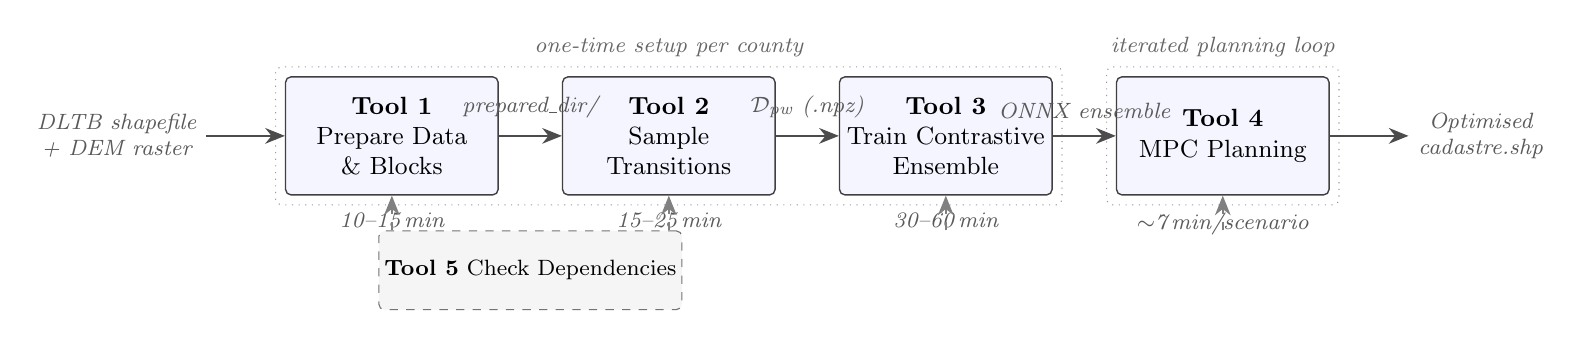
\begin{tikzpicture}[
  font=\small,
  node distance=6mm and 8mm,
  tool/.style={rectangle, rounded corners=2pt, draw=black!75, line width=0.5pt,
               minimum width=27mm, minimum height=15mm, align=center,
               fill=blue!4, inner sep=2pt},
  io/.style={font=\footnotesize\itshape, text=black!65, align=center},
  flow/.style={-{Stealth[length=2.5mm,width=2mm]}, line width=0.6pt, draw=black!70},
  check/.style={rectangle, rounded corners=2pt, draw=black!55, dashed, line width=0.4pt,
                minimum width=27mm, minimum height=10mm, align=center,
                fill=gray!8, inner sep=2pt, font=\footnotesize}
]
% Inputs
\node[io] (in) {DLTB shapefile\\+ DEM raster};

% Four tools left to right
\node[tool, right=10mm of in]              (t1) {\textbf{Tool 1}\\Prepare Data\\\& Blocks};
\node[tool, right=of t1]                   (t2) {\textbf{Tool 2}\\Sample\\Transitions};
\node[tool, right=of t2]                   (t3) {\textbf{Tool 3}\\Train Contrastive\\Ensemble};
\node[tool, right=of t3]                   (t4) {\textbf{Tool 4}\\MPC Planning};

% Output
\node[io, right=10mm of t4] (out) {Optimised\\cadastre.shp};

% Inter-tool I/O hints (above each arrow)
\node[io, above=1mm of $(t1)!0.5!(t2)$] {prepared\_dir/};
\node[io, above=1mm of $(t2)!0.5!(t3)$] {$\mathcal{D}_{\text{pw}}$ (.npz)};
\node[io, above=1mm of $(t3)!0.5!(t4)$] {ONNX ensemble};

% Wall-time hints (below)
\node[io, below=1mm of t1] {10--15\,min};
\node[io, below=1mm of t2] {15--25\,min};
\node[io, below=1mm of t3] {30--60\,min};
\node[io, below=1mm of t4] {$\sim$7\,min/scenario};

% Flow arrows
\draw[flow] (in)--(t1);
\draw[flow] (t1)--(t2);
\draw[flow] (t2)--(t3);
\draw[flow] (t3)--(t4);
\draw[flow] (t4)--(out);

% One-time vs iterated bracket
\begin{scope}[on background layer]
\node[draw=black!40, dotted, rounded corners=2pt, line width=0.4pt,
      fit=(t1)(t2)(t3),
      label={[font=\footnotesize\itshape, text=black!60]above:one-time setup per county}] (setup) {};
\node[draw=black!40, dotted, rounded corners=2pt, line width=0.4pt,
      fit=(t4),
      label={[font=\footnotesize\itshape, text=black!60]above:iterated planning loop}] (plan) {};
\end{scope}

% Tool 5 sidecheck
\node[check, below=12mm of $(t1)!0.5!(t2)$] (t5) {\textbf{Tool 5} Check Dependencies};
\draw[flow, dashed, draw=black!50] (t5.north -| t1.south) -- (t1.south);
\draw[flow, dashed, draw=black!50] (t5.north -| t2.south) -- (t2.south);
\draw[flow, dashed, draw=black!50] (t5.north -| t3.south) -- (t3.south);
\draw[flow, dashed, draw=black!50] (t5.north -| t4.south) -- (t4.south);

\end{tikzpicture}%
}
\caption{The four-tool ArcGIS Pro deployment pipeline (\S\ref{sec:methods-toolchain}). Tools~1--3 run once per county to prepare cadastral data, sample the pairwise dataset, and train the contrastive transition-model ensemble (exported to ONNX). Tool~4 is the iterated planning loop a county officer runs repeatedly under different reward weightings; one 100-step scenario finishes in $\sim$7\,min on a desktop CPU. A separate Tool~5 (dashed) validates the Python environment, Spatial Analyst availability, and ONNX shape compatibility before any pipeline run is allowed.}
\label{fig:toolchain}
\end{figure}

The runtime profile reflects a deliberate split between one-time setup (Tools 1--3, $\sim$1--2\,h on a 12-thread CPU per county) and repeated planning (Tool 4, $\sim$7\,min per scenario). An end-to-end UI-driven run on full Bishan, with the same training data and hyperparameters as Section~\ref{sec:counties}, yields a slope improvement of $-1.544 \pm 0.041\%$ across five evaluation episodes of the shipped Bishan ensemble (same direction and order of magnitude as the lab figure of $-1.289 \pm 0.079\%$; the gap reflects two replication regimes, 5 ensembles × 1 episode in the lab versus 1 ensemble × 5 episodes in the toolchain). To support users without an ArcGIS Pro license, the same end-to-end pipeline is also exposed through a non-commercial command-line interface (\texttt{farmland-mpc prepare/sample/train/plan}) that runs against any QGIS-compatible vector and raster stack via \texttt{geopandas}/\texttt{rasterio}. The package is released under MIT licence; the synthetic benchmark (Section~\ref{sec:bench}) under CC-BY 4.0. Together with the trained Bishan ensemble and the released restoration cases (\S\ref{sec:cross-domain}), this forms a complete reproduction kit usable on either ArcGIS Pro or a free QGIS-compatible Python environment.

% ============================================================================
\section{Discussion}\label{sec:discussion}
% ============================================================================

\paragraph{What the pipeline delivers for sustainability planning.} For consolidation policy in mountainous-terrain counties, the operational shift is qualitative. Model-free reinforcement-learning baselines previously required $8$--$12$ GPU-hours per scenario and collapsed on roughly a quarter of attempted runs; classical operations-research methods at the same wall-clock budget reach less than $11\%$ of contrastive MPC's reward on Bishan. With contrastive MPC, a planner obtains a scenario in $\sim$7 minutes on a desktop, with cross-seed variance several-fold smaller than DRL baselines. What changes is what becomes routine: a planning office can explore dozens of weight settings, township sub-budgets, or red-line constraints in a working day. The honest area trade-offs we document are themselves first-order useful: the agent's behaviour is morphology-dependent, so scenario exploration is not optional.

\paragraph{Methodological mechanism.} The dominant obstacle to learned-model planning was a single feature of the standard training objective: mean-squared-error loss on the reward head learns the average of the per-state reward distribution but not its rank order across actions. A learned model can therefore look excellent on every standard fidelity metric while giving $51.6\%$ pairwise ranking accuracy. Adding a single auxiliary pairwise large-margin term closes this gap without architectural change. This intervention is conditional rather than universal: it is needed when within-state action variance is small relative to between-state variance ($\sigma_a / \sigma_s \lesssim 1$, the regime to which farmland's geometric reward function belongs), and is redundant when reward is a per-unit attribute lookup. The learned-surrogate pipeline as a whole, separately, beats classical operations-research baselines (greedy, simulated annealing, NSGA-II, MILP) when each simulator step is computationally expensive ($\geq 30$\,ms in our measurements) or when reward exhibits combinatorial cost interactions, or both---farmland satisfies both conditions, the empirical reason the pipeline dominates farmland but not restoration default.

\paragraph{Practical implication for problem selection.} Practitioners considering a learned-surrogate planner on a new domain should report two quantities: simulator step cost (in ms/step) and whether reward exhibits combinatorial cost interactions. When step cost exceeds $\sim 30$\,ms or combinatorial structure is non-trivial, the learned-surrogate pipeline is in the advantage regime; otherwise well-tuned classical methods reach near-optimum at lower wall-clock cost. We expect this criterion to extend to applications where high-fidelity physics simulators dominate per-step cost: hydrologic-model-driven watershed restoration, integrated power-grid maintenance scheduling, multi-stage chemical-reaction prioritisation, and supply-chain optimisation under economic-equilibrium models all combine non-trivial step cost with combinatorial constraint structure.

\paragraph{Bounds on the claim.} Four constraints qualify the result. Cadastral evidence comes from two counties in southwestern China within the same regional regime; structurally different agricultural settings remain untested as far as the contrastive intervention is concerned, although the cross-domain restoration cases (\S\ref{sec:cross-domain}) demonstrate that the underlying \emph{diagnostic} extends beyond the farmland regime even when the intervention itself does not. A finer characterisation across the variance ratio $\sigma_a^2 / \sigma_s^2$ would let practitioners decide a priori whether to add the auxiliary loss. The pairwise dataset relies on simulator snapshot/restore, available in our gridded simulators but not in many physics-based environments. Hyperparameter sweeps are coarse; finer resolution may yield further improvement but is not expected to reverse the qualitative ordering. Three follow-ups are immediate: regime-broadening to combinatorial planning problems with high simulator cost outside spatial-cadastral domains; per-objective ranking that lets planners use objective-specific scoring as a deployment lever; offline planning with contrastive-trained ensembles at policy-relevant horizons.

% ============================================================================
\section*{Methods}
\label{sec:methods}
% ============================================================================

\paragraph{Scope and architectural framing.} The architecture used throughout this paper is a feed-forward deterministic learned transition model with a discriminative reward head (\S\ref{sec:methods-action} below). It is in the operational sense of \citet{chua2018deep} and \citet{janner2019trust} a learned $\hat{p}(s_{t+1}, r_t \mid s_t, a_t)$ that substitutes for the real environment in MPC lookahead and dream-style policy training; it is not a generative world model in the contemporary Dreamer sense \citep{hafner2025dreamerv3,ha2018world}. The task is fully observed (state is the per-block 17-dim feature vector emitted by Tool 1; no raw observation), episodic (100-step cap, no partial observability), and the action space is finite categorical of size $N_{\text{blocks}}$ (Methods, \S\ref{sec:methods-action}); we therefore do not learn a state representation from raw observations and do not use recurrent latent dynamics (RSSM). Combining a learned state encoder with the ranking-loss head reported here is a natural extension for settings where partial observability or pixel-level inputs apply (\S\ref{sec:discussion}).

\subsection*{Per-parcel slope from DEM and cadastral polygons}\label{sec:methods-prepare}

The per-parcel slope feature used throughout the analysis is derived from the Third National Land Survey cadastral polygons and Copernicus DEM GLO-30 elevation tiles \citep{copernicus2021dem}, both freely available in their respective public archives. The DEM is kept in its native geographic CRS (EPSG:4326, 1-arcsecond resolution); slope is computed by central-difference gradients on the elevation grid using true east-west and north-south metres-per-pixel obtained from \texttt{pyproj.Geod} (WGS84 ellipsoid) at the study-area centre latitude. The pixel spacing is $\sim$$27$\,m east-west and $\sim$$31$\,m north-south at $29.5^\circ$N (the centre of both Bishan and Neijiang); reprojecting the DEM to a metric projection before gradient differencing would average over these non-square cells and systematically under-estimate slope. The slope raster, in degrees, is then aggregated to each cadastral polygon by area-weighted zonal mean over all DEM cells whose centre falls within the polygon. Polygons that contain no cell centre (typically very small parcels, $\lesssim 30$\,m linear scale) inherit the per-county median slope to keep the downstream feature vector finite; on Bishan and Neijiang this affects $\sim$$2$\% and $\sim$$3$\% of parcels respectively, all in the smallest size class. The full prepare pipeline (DEM merge $\to$ slope $\to$ zonal mean $\to$ per-township block construction) takes $\sim$$3$ minutes on Bishan and $\sim$$5$ minutes on Neijiang on a 14-core desktop CPU and is released as the \texttt{farmland-mpc prepare} command (\S Code Availability).

\subsection*{Problem setting and action-space encapsulation}\label{sec:methods-action}

We study county-level farmland consolidation in two real counties (Bishan District, Chongqing; Neijiang Dongxing District, Sichuan) and seven synthetic landscapes (\S\ref{sec:methods-synth}). For Bishan, the planning area comprises 13 townships, $2{,}600$ spatial blocks, and $52{,}515$ cadastral parcels; for Neijiang, 29 townships, $3{,}711$ blocks, and $76{,}376$ parcels (Table~\ref{tab:counties}). Each block aggregates multiple parcels and is characterised by 17 features (farmland area, forest area, slope statistics, adjacency metrics, and investment indicators). Global context is encoded as an additional 12 features (remaining budget, contiguity, \textit{baimu fang} count, etc.). The episode length is fixed at 100 steps for the real-data experiments and 50 steps for the synthetic benchmark (\S\ref{sec:bench}); each step has a budget of up to 5 paired farmland--forest swaps.

\paragraph{Agent action space.}
The agent's action space is a single categorical choice over the spatial blocks per step: $a_t \in \{1, \ldots, N_{\text{blocks}}\}$. The agent does \emph{not} select individual parcels or the paired-swap sub-actions. Given the selected block, the environment internally executes \emph{up to} 5 paired farmland--forest swaps within that block using a deterministic rule-based procedure: candidate pairs are enumerated by joint feasibility under the farmland-red-line and slope constraints, scored by a local improvement heuristic, and the top-scoring feasible pairs are applied until either 5 pairs are executed or the candidate pool is exhausted. The agent therefore chooses \emph{where} to act, not \emph{what} to do within the chosen location; this encapsulation keeps the action space at a tractable scale ($\sim 10^3$) while preserving the paired-swap semantics that respect the farmland-area red line (total farmland area is conserved as land moves between farmland and forest classes rather than being removed outright).

\paragraph{Action masking.}
Not all blocks are legal targets at every step. The action mask $m_t \in \{0, 1\}^{N_{\text{blocks}}}$ disables blocks that (i) have no remaining feasible parcel pairs (either exhausted in earlier steps or structurally infeasible under the red-line/slope constraints), (ii) are currently in a township whose per-township swap budget has been exhausted, or (iii) have been selected in the immediately previous step (a simple debounce to prevent action thrashing). MaskablePPO \citep{ross2011reduction,schulman2017proximal,huang2022maskable}-style masking is applied in both the policy sampling and the MPC candidate enumeration, so that illegal blocks have zero probability or are excluded from the $K$ candidate set.

\subsection*{Reward formulation}\label{sec:methods-reward}

Each step's reward combines three normalised directional signals (slope, contiguity, and qualifying-patch area), a large-patch formation bonus, and an asymmetric area-protection penalty. Let $\bar{\sigma}_t$ be the area-weighted mean farmland slope at step $t$, $C_t$ the within-farmland contiguity index, $B_t$ the count of qualifying \textit{baimu fang} ($\geq$6.67\,ha contiguous farmland patches), and $A_t$ their total area. The per-step reward is
\begin{equation}
\label{eq:reward}
r_t \;=\; w_S \cdot \Delta \bar{\sigma}_t
       \;+\; w_C \cdot \Delta C_t
       \;+\; w_A \cdot \Delta A_t
       \;+\; b_B \cdot \max(0,\, B_t - B_{t-1})
       \;+\; p_A \cdot \min(0,\, \Delta A_t)
\end{equation}
where the directional changes are normalised by their initial county-wide values: $\Delta \bar{\sigma}_t = (\bar{\sigma}_{t-1} - \bar{\sigma}_t)/\bar{\sigma}_0$ (so that slope \emph{reduction} contributes positively), $\Delta C_t = (C_t - C_{t-1})/C_0$, and $\Delta A_t = (A_t - A_{t-1})/A_0^{\mathrm{farm}}$ (normalised by the initial total farmland area $A_0^{\mathrm{farm}}$, so the weights act on relative rather than absolute changes). Weights $(w_S, w_C, w_A, b_B, p_A) = (4000, 500, 1500, 5, 2000)$ are inherited from our in-house DRL baseline configuration. The fourth term is a one-off bonus applied each time the qualifying-patch count increases between steps; the fifth term, $p_A \cdot \min(0, \Delta A_t)$, is an asymmetric penalty that activates only when qualifying area decreases, roughly doubling the marginal cost of shedding \textit{baimu fang} area relative to the symmetric $w_A$ reward (this asymmetry is what drives the agent to consolidate many small qualifying patches into fewer larger ones, increasing total qualifying \emph{area} even as the qualifying \emph{count} falls; \S\ref{sec:counties}). Under a median single-step decomposition, slope improvement contributes $\sim$60\%, contiguity $\sim$15\%, qualifying-patch area $\sim$20\%, and the formation bonus $\sim$5\%. We did not re-tune the weights for the present experiments; contrastive MPC, dream-trained PPO, and the model-free baselines all use the identical reward function, so any method-wise difference is attributable to the learning procedure rather than to reward engineering. A separate fixed penalty of $-1$ is applied whenever a selected block admits no feasible paired swap, discouraging wasted actions. Throughout the paper, ``Slope \%'' is the relative change $\text{Slope \%} = (\bar{\sigma}_T - \bar{\sigma}_0)/\bar{\sigma}_0 \times 100$; contiguity and \textit{baimu fang} count/area changes are absolute.

\subsection*{Block-level transition model}

The transition model is a feed-forward neural network with approximately $237{,}000$ parameters that takes as input the current block features (all blocks, 17 dimensions each), the global features (12 dimensions), and the selected action (block index), and predicts the next-step block features, global features, and scalar reward. Only the selected block changes (residual formulation). The base loss is
\begin{equation}
\mathcal{L}_{\text{MSE}} = \mathrm{MSE}(\Delta\hat{b}, \Delta b) + \mathrm{MSE}(\Delta\hat{g}, \Delta g) + 0.1 \cdot \mathrm{MSE}(\hat{r}, r),
\end{equation}
trained with Adam (learning rate $10^{-3}$, weight decay $10^{-5}$) on a 90/10 train/validation split with patience-6 early stopping.

\subsection*{Ensemble uncertainty estimation}

We train 3--5 independently initialised transition models on the same dataset with different random seeds \citep{lakshminarayanan2017simple}. At inference, the ensemble produces mean predictions for next state and reward, plus the reward standard deviation $\sigma_r$ across members. The dream environment penalises high-disagreement actions: $r_{\text{out}} = \bar{r} - \lambda_{\text{disag}} \cdot \sigma_r$ with $\lambda_{\text{disag}} = 0.5$.

\subsection*{Policy architecture: parcel-scoring policy}

The policy is a dimension-invariant scoring network compatible with MaskablePPO. For each block $i$, the scorer concatenates the block's 17-dimensional local features with the 12-dimensional global state, passes the result through a shared MLP ($[64, 32] \to 1$), and produces a scalar score. The action is the highest-scoring valid block. A separate value network takes only the global features and predicts the state value.

\subsection*{DAgger-style iterative refinement}

We adopt a DAgger-style loop \citep{ross2011reduction}: (1)~collect an initial dataset $D_0$ of $6{,}000$ transitions from random and greedy policies on the real environment; (2)~train the transition model ensemble on $D_{\leq i}$; (3)~train a policy in the dream environment for $50{,}000$ timesteps; (4)~evaluate on the real environment; (5)~collect 10 stochastic on-policy episodes ($\sim$$1{,}000$ transitions) and augment the dataset. Three iterations are performed.

\subsection*{Targeted evidence collection and stabilisation}

In targeted DAgger, step (5) above is modified: each transition is scored by ensemble reward disagreement $\sigma_r$, and only transitions exceeding threshold $\tau = 0.5$ are retained; under this threshold, $\sim$$99.6\%$ of transitions are filtered out, accounting for the dream-policy slowdown documented in \S\ref{sec:rank}. Three stabilisation mechanisms are applied across all protected runs. \emph{Best-checkpoint selection}: every $10{,}000$ PPO timesteps, the current policy is evaluated on the real environment (3 episodes); the checkpoint with the highest mean reward is retained. \emph{Iteration-1 rollback}: if iteration-1 reward drops more than 50 points below iteration-0, the dataset and policy are reverted. \emph{Early stopping}: training halts if validation loss does not improve for 6 consecutive epochs.

\subsection*{Model-predictive planning protocol}\label{sec:methods-mpc}

We use random shooting model-predictive control \citep{garcia1989model,williams2017model,rubinstein1999cross}. At each real-environment step $t$ with state $s_t$:
\begin{enumerate}
\item Sample $K$ random action sequences $\{a^{(k)}_{t:t+H-1}\}_{k=1}^K$, each of length $H$, from the action-masked support.
\item For each sequence, roll forward through the ensemble mean model: $\hat{s}^{(k)}_{t+1}, \hat{r}^{(k)}_t = f_\theta(s_t, a^{(k)}_t)$, continuing autoregressively for $H$ steps.
\item Score each sequence by cumulative predicted reward: $R^{(k)} = \sum_{h=0}^{H-1} \hat{r}^{(k)}_{t+h}$.
\item Execute $a^{(k^*)}_{t}$ where $k^* = \arg\max_k R^{(k)}$ on the real environment.
\item Advance to $s_{t+1}$ (real) and repeat.
\end{enumerate}
For the synthetic-benchmark sweep (\S\ref{sec:bench}), the same protocol is applied with $H{=}5$, $K{=}50$, and greedy continuation (each subsequent step within a sequence picks the predicted-reward argmax over $50$ candidates rather than continuing the random rollout). This is the configuration that becomes optimal under the contrastive ensemble (Table~\ref{tab:contrastive-mpc}).

\subsection*{Aggregate fidelity vs within-state action ranking under MSE training}\label{sec:methods-fidelity-vs-ranking}

The decoupling described in \S\ref{sec:rank} is a property of the loss. Let $\hat{r}_\theta(s, a)$ be the reward head of a learned model trained on $(s, a, r)$ pairs from a distribution $\mu(s, a)$, and let
\begin{equation}
\mathcal{L}_{\text{MSE}}(\theta) \;=\; \mathbb{E}_{(s,a)\sim\mu}\big[(\hat{r}_\theta(s,a) - r(s,a))^2\big]
\end{equation}
be the standard objective. Two distinct quantities can be evaluated on this learned model: \emph{aggregate fidelity}, defined as the population MSE itself, and \emph{within-state ranking accuracy}
\begin{equation}
\mathcal{A}_{\text{rank}}(\theta) \;=\; \mathbb{E}_{s\sim\mu_s}\,\mathbb{E}_{a_i,a_j\sim\mu(\cdot \mid s)}\!\left[\mathbf{1}\big[\mathrm{sign}(\hat{r}_i - \hat{r}_j) = \mathrm{sign}(r_i - r_j)\big]\right],
\end{equation}
which is the quantity model-predictive top-$K$ selection actually consumes when scoring action menus at a single environment state.

The two quantities are not constrained against each other under MSE training. Consider a setting in which, at every state $s$, the action-conditioned reward distribution is symmetric around a state-dependent mean $\bar{r}(s)$ with state-marginal variance $\sigma_s^2$ and within-state action variance $\sigma_a^2(s)$. The learned predictor $\hat{r}_\theta^{\star}(s,a) = \bar{r}(s)$, which assigns the conditional mean to every action regardless of its identity, achieves population MSE equal to $\mathbb{E}_s[\sigma_a^2(s)]$ (the irreducible state-conditional variance) and within-state ranking accuracy equal to $1/2$ on every pair with non-zero true reward difference, identical to random guessing. A learned model can therefore minimise MSE within a constant of the Bayes optimum while remaining indistinguishable from random on the very ranking decisions that drive planning. Our $51.6\%$ rank accuracy at cosine similarity $0.998$ is empirically close to this regime: the predicted reward standard deviation across the action menu (Table~\ref{tab:contrastive-disc}) is compressed by an order of magnitude relative to the true within-state variance, exactly as the conditional-mean predictor would behave. This is a counterexample showing MSE \emph{does not guarantee} ranking fidelity in regimes where $\sigma_a^2(s) \ll \sigma_s^2$, not a statement of statistical independence: in regimes where $\sigma_a^2(s)$ is large relative to $\sigma_s^2$, MSE training will in practice acquire much of the ranking signal as a by-product (\S\ref{sec:cross-domain} demonstrates this empirically).

\subsection*{Contrastive training protocol}\label{sec:methods-contrastive}

\paragraph{Pairwise data generation.} We sample states by rolling out random trajectories in the real CountyLevelEnv. At each step, we (i)~snapshot the full environment state (land-use assignments, swap counts, block availability caches, running slope/contiguity sums; 19 attributes total), (ii)~sample 50 valid actions uniformly from the action mask, (iii)~execute each action from the snapshotted state, recording the immediate reward, and (iv)~restore the snapshot before advancing with a fresh random action. We continue across multiple episodes until $1{,}000$ states are collected, yielding $50{,}000$ ground-truth $(s, a, r)$ evaluations. The pairwise dataset $\mathcal{D}_{\text{pw}}$ is saved as $(s_i, \{a_{i,j}\}_{j=1}^{50}, \{r_{i,j}\}_{j=1}^{50})$ for $i = 1, \ldots, 1000$. Generation took 45 minutes on commodity CPU hardware. Snapshot/restore is a simulator-specific capability; replay-buffer substitutes are an open question (Limitations).

\paragraph{Loss function.} The augmented training objective adds a margin ranking term:
\begin{equation*}
\mathcal{L}_{\text{rank}} = \mathbb{E}_{(s_i, a_{i,j}, a_{i,k}) \sim \mathcal{D}_{\text{pw}}} \left[ \max\left(0, -\sigma_{jk} \cdot (\hat{r}_{i,j} - \hat{r}_{i,k}) + m\right) \right]
\end{equation*}
where $\sigma_{jk} = \text{sign}(r_{i,j} - r_{i,k}) \in \{-1, 0, +1\}$ is the ground-truth pairwise label, $m = 0.1$ is the margin, and pairs with $\sigma_{jk} = 0$ are excluded. At each training step, we sample 10 action pairs per state from 50--100 randomly selected pairwise-dataset states. Total objective: $\mathcal{L} = \mathcal{L}_{\text{MSE}} + \lambda_{\text{rank}} \mathcal{L}_{\text{rank}}$.

\paragraph{Margin choice.} The margin $m = 0.1$ is approximately $1/8$ of the empirical ground-truth reward standard deviation ($0.811$ on $\mathcal{D}_{\text{pw}}$). A coarse sweep of $m \in \{0.05, 0.1, 0.2\}$ on a held-out validation fold showed a flat optimum: ranking accuracy at $\lambda_{\text{rank}}{=}5.0$ varied within $\pm 1.5$ percentage points across these three choices.

\paragraph{Training.} We use 3-member ensembles trained with Adam ($\text{lr}=10^{-3}$, weight decay $10^{-5}$), batch size 256, for 15 epochs with patience 20. Each ensemble trains in $\sim$25 minutes on commodity CPU hardware. We sweep $\lambda_{\text{rank}} \in \{0.0, 1.0, 5.0\}$ using an 80/20 train/validation split of the pairwise dataset. MPC evaluation uses $H{=}5$, $K{=}50$, greedy continuation with $50$ candidates per continuation step.

\subsection*{Synthetic benchmark generator}\label{sec:methods-synth}

The seven synthetic landscapes used in Section~\ref{sec:bench} are produced by a deterministic, seed-controlled generator that reads a YAML preset (terrain type, target block count, parcel-density distribution, land-use fractions, fragmentation length-scale, seed) and emits a directory of GeoJSON, CSV, GeoTIFF, and JSON files identical in schema to the real-data preprocessor's outputs. The generator is fully deterministic given $(\text{preset}, \text{seed})$.

\paragraph{Eight-stage pipeline.} (1)~\emph{Domain tessellation}: Voronoi tessellation of $n_{\text{blocks}}$ seeds in a rectangle of suitable extent (size driven by parcels-per-block target). (2)~\emph{DEM synthesis}: 2D Perlin noise with multi-octave fractal terrain, preset-controlled amplitude and length-scale, clipped to non-negative. (3)~\emph{Slope derivation}: Horn's algorithm on the synthetic DEM, sampled to each block as area-weighted mean and max. (4)~\emph{Parcel subdivision within blocks}: secondary Voronoi inside each block polygon using the parcels-per-block distribution. (5)~\emph{Land-use assignment}: a Gaussian random field thresholded into farmland / forest / other classes, with preset-controlled length-scale driving fragmentation. (6)~\emph{Feature computation}: 17-dim block feature vectors using the same code path as the real-data \texttt{county\_env.py} (farmland area, forest area, slope statistics, adjacency features), guaranteeing environment compatibility. (7)~\emph{Adjacency graph}: planar adjacency from shared block edges, with median degree close to the preset target. (8)~\emph{Posterior calibration check} (anchors only): compute initial slope, contiguity, \textit{baimu fang} count, and \textit{baimu fang} area, and verify within $\pm 50\%$ of the real anchor values; deviations are surfaced in a calibration delta report rather than silently accepted.

\paragraph{Dual-anchor calibration.} Two of the seven presets, \texttt{bishan\_clone} and \texttt{neijiang\_clone}, are calibrated against Bishan and Neijiang respectively such that any single seed reproduces the four headline initial-state metrics within $\pm 50\%$ of the real anchor. The other five presets vary morphology along terrain, size, and fragmentation axes (\S\ref{sec:bench}) but are not constrained against any real anchor; they are parameter-controlled stress tests rather than evidence of regional generalisation. Contiguity is the weakest calibration axis ($\sim$$6\%$ on Bishan clone, $\sim$$44\%$ on Neijiang clone), reflecting Voronoi-based geometries' tendency to be more uniformly contiguous than real cadastre shaped by ridges, roads, and water channels.

\paragraph{Compatibility shim.} A thin \texttt{synthetic\_env\_loader.py} reads the generator outputs (\texttt{blocks.csv} + \texttt{adjacency.json}) and returns the same data structure that \texttt{county\_env.py} expects from real data; no environment-code changes are required. The synthetic and real evaluation regimes therefore use identical simulator semantics, ensuring that any cross-regime difference is attributable to the landscape, not to the engine.

\subsection*{Restoration-prioritisation env (cross-domain verification)}\label{sec:methods-restoration}

The cross-domain verification of \S\ref{sec:cross-domain} reuses the entire farmland pipeline (sample, train, plan) by swapping only the env class and the per-unit feature vector. The restoration env is a finite-action gymnasium environment over $n_{\text{units}}$ planning cells; the action space is $\{0, 1, \ldots, n_{\text{units}}-1\}$, and ``select unit $a$'' is a one-time monotonic assignment (no swap, no reversibility). The action mask excludes already-selected units and units whose individual restoration cost would exceed the remaining budget. The reward at step $t$ when selecting unit $a_t$ is a fixed linear combination
\begin{equation*}
r_t \;=\; \sum_{k} w_k \cdot \phi_k(a_t)\;+\;w_{\text{conn}} \cdot \frac{|\{j \in \mathcal{N}(a_t):\,j\text{ already selected}\}|}{|\mathcal{N}(a_t)|}\;-\;w_{\text{cost}} \cdot \frac{c(a_t)}{B}
\end{equation*}
where $\phi_k$ are per-unit attribute scores read from a CSV (risk index, water-quality priority, biodiversity, etc.), $w_k$ are weights specified in a per-case scenario configuration file, $\mathcal{N}(a_t)$ is the queen-contiguity neighbour set, $c(a_t)$ is the unit's restoration-cost proxy, and $B$ is the cumulative budget. State features $b \in \mathbb{R}^{n_{\text{units}} \times 17}$ are the standardised per-unit attributes (zero-padded to match $K_{\text{block}}=17$ so the same network architecture as farmland applies); the global state $g \in \mathbb{R}^{12}$ encodes fraction-of-budget-remaining, fraction-of-units-selected, fraction-of-steps-elapsed, and per-component cumulative reward. Snapshot/restore is implemented by capturing the boolean selection mask, cumulative reward components, budget used, and step counter; the env is purely combinatorial and has no expensive-to-restore geometric state, so pairwise dataset generation runs in seconds rather than minutes.

For the Buchanan VA case ($n_{\text{units}}=562$), per-unit features are derived from the OSMRE e-AMLIS national abandoned-mine-lands inventory \citep{osmre2019eamlis}, USGS NHD flowline data \citep{usgs2024nhd}, USGS 3DEP elevation \citep{usgs2024_3dep}, and Census TIGER county boundaries \citep{census2023tiger}, all freely available as public open data; episode length is 50 steps and the cumulative cost cap is set to \$200{,}000 in notional cost-proxy units. The cost-proxy field is derived as \texttt{restoration\_cost\_proxy} = unit area in hectares (rescaled by 10), which yields a roughly e-AMLIS-comparable ranking among units but should not be interpreted as a real-world dollar reclamation cost; the e-AMLIS unfunded-cost field is sparse and unevenly populated across the inventory, and we therefore use a transparent area-based proxy and report results in proxy units rather than claim a calibrated cost-benefit analysis. For the synthetic case ($n_{\text{units}}=420$), feature, adjacency, and reward generators are deterministic given a seed and are released alongside the synthetic benchmark of \S\ref{sec:bench}; episode length is 60 steps and the cost cap is 45{,}435 in synthetic units (no real-world correspondence). Both cases share the same MPC configuration as farmland ($H{=}5$, $K{=}50$, greedy continuation, scoring=reward) and the same training hyperparameters ($\lambda_{\text{rank}}{=}5.0$ for contrastive, margin $0.1$, three-member ensembles per seed, five seeds for both the contrastive ($\lambda{=}5$) and the MSE-only ($\lambda{=}0$) conditions to ensure a fair head-to-head comparison.

The cumulative wall-clock for the full restoration verification (two cases, one prepare each, one sample each, six ensemble trains per case, six MPC plans, one random baseline per case) is approximately 30 minutes on a 14-core M-series Apple Silicon CPU running 3 ensembles in parallel; the cases are released as part of the open reproduction kit (\S Code Availability).

\subsection*{Simulator-cost crossover protocol}\label{sec:methods-simcost}

The simulator-cost analysis of \S\ref{sec:simcost} treats the per-step wall cost of \texttt{env.step} as an independent variable. To isolate it from confounds (action space size, reward function, optimisation algorithm), we instrument the restoration env's reward dispatcher with a configurable \texttt{time.sleep(delay\_s)} call invoked exactly once per \texttt{env.step}. We then run two algorithms at matched 30\,s wall budgets across delays $d \in \{0, 1, 10, 50, 100\}$\,ms.

\paragraph{Simulated-annealing baseline.} We run a permutation-space SA over the candidate-unit action ordering. Each iteration: sample $i, j \in \{0, \ldots, 79\}$ uniformly; swap positions $i$ and $j$ in the current ordering; re-roll out the full episode; accept the swap if it improves the cumulative reward, or with probability $\exp(\Delta r / T_t)$ otherwise; geometrically cool $T_t$ at rate $0.995$. Initial ordering is the priority-score-greedy ordering (this gives SA a strong warm start). The number of iterations actually completed within the 30\,s wall budget is the diagnostic: at delay 0 it reaches $\sim 9{,}000$, at delay $100$\,ms it reaches $\sim 6$.

\paragraph{Learned-surrogate MPC baseline.} We run \texttt{mpc\_select\_action} with random continuation, $H{=}5$, $K{=}50$, $\gamma{=}0.99$, scoring=reward, on each of the seeded RNG paths $\{1, 18, 35, \ldots\}$ until the wall budget is exhausted. We report the best cumulative episode reward seen. The per-step ensemble forward pass is $\sim 25$\,ms (one batched ONNX call evaluating all $K{=}50$ candidates in parallel) and is decoupled from the injected \texttt{env.step} delay; only the eventual environment commit step pays the simulator cost.

\paragraph{Farmland baseline measurement.} The farmland Bishan datapoint (Figure~\ref{fig:simcost}, gold star) is measured on the actual CountyLevelEnv without any injected delay. The natural step cost is profiled as $17.9 \pm 0.3$\,ms over a 5-step probe repeated three times (the variance is dominated by per-step \textit{baimu fang} cache hits / misses; in the worst case where the union-find aggregation triggers, single-step cost rises to $\sim 60$\,ms). Under a 180\,s wall budget rather than 30\,s (chosen because the wall cost per SA iteration on farmland is $\sim 1.8$\,s, so 30\,s would only allow $\sim 16$ iterations and SA would not even reach its initial cooling regime), simulated annealing reaches reward $9.04$ at $n_{\text{iter}}=100$, random restart over 98 episodes reaches $30.85$, and contrastive MPC reaches $86.74$. The full driver script is released in \texttt{farmland\_mpc/tests/farmland\_baselines.py}.

\subsection*{ArcGIS Pro toolchain}\label{sec:methods-toolchain}

The deployment artefact described in \S\ref{sec:deploy} is an ArcGIS Pro Python Toolbox (\texttt{LandUseOptimization\_P9.pyt}) exposing five tools: \emph{(1)~Prepare Data \& Blocks} ingests a Third National Land Survey \texttt{DLTB} shapefile and a digital elevation model and emits the block-level state expected by the learned-model code; \emph{(2)~Sample Transitions} generates the pairwise dataset $\mathcal{D}_{\text{pw}}$ on the user's data via the snapshot/restore protocol described above; \emph{(3)~Train Contrastive Ensemble} trains a 3-member ensemble at $\lambda_{\text{rank}}{=}5.0$ and exports each model to ONNX with the user's $N_{\text{blocks}}$ baked in; \emph{(4)~MPC Planning} runs the planning loop and writes back an optimised cadastral shapefile readable by any standard GIS workflow; \emph{(5)~Check Dependencies} validates the user's Python environment (ArcGIS Pro 3.6+, Spatial Analyst extension, \texttt{gymnasium}, \texttt{libpysal}) before any pipeline run is permitted. Tools 1--3 are run once per county on commodity desktop hardware ($\sim$1--2 hours total wall time); Tool 4 is the iterated planning loop (one $\sim$7-minute scenario per call). A 70-second smoke test on a 2-township subset of Neijiang Dongxing District completes the full pipeline as a continuous-integration check.

Two operational caveats are visible in the toolchain. First, the ONNX export bakes in $N_{\text{blocks}}$, so a pre-trained ensemble cannot be reused across counties; Tool 4 carries an explicit pre-flight check that refuses to run if the pre-trained ensemble's $N_{\text{blocks}}$ does not match the prepared dataset. Second, the default projected coordinate reference system (\texttt{EPSG:32648}, UTM zone 48N) covers central and western China; users in eastern, north-eastern, or north-western China must override the projection in Tool 1 to avoid slope errors. The end-to-end Bishan replication on the toolchain achieves a slope improvement of $-1.5439 \pm 0.0409\%$ (1 shipped ensemble, 5 episodes), modestly below the lab-pipeline figure of $-1.289 \pm 0.079\%$ (5 independently trained ensembles, 1 episode each); we report the gap honestly rather than tune it away.

\subsection*{Evaluation protocol}

For the real-data experiments (\S\ref{sec:counties}), each configuration is evaluated with 5 deterministic episodes on the real CountyLevelEnv. Reported metrics include mean reward, slope change ($\%$), contiguity change, \textit{baimu fang} count change, and total \textit{baimu fang} area change. For the synthetic benchmark (\S\ref{sec:bench}), each method is run for 5 random seeds on each of the 7 presets; per-cell results are aggregated as cross-seed mean $\pm$ sample standard deviation. Cross-seed statistics for the contrastive configurations are computed across 5 independently trained ensembles (different random seeds for both the pairwise dataset and the network initialisation). Statistical tests against fixed baseline values are one-sample $t$-tests; tests between two methods on matched seeds use paired $t$-tests and Wilcoxon signed-rank tests. We report test type, df, $p$, and Cohen's $d$ throughout.

\subsection*{Independent GIS-grounded verification of reported gains}\label{sec:methods-validate}

Because the headline metrics in \S\ref{sec:counties} are computed inside the same CountyLevelEnv whose learned ensemble drives the MPC scoring loop, a sceptical reviewer can ask whether the reported slope reduction is a real change in the optimised cadastre or an artefact of the learned dynamics agreeing with the planner. To resolve this, we recompute all three primary metrics directly from the optimised DLTB shapefile written to disk by Tool~4, using a 190-line script that depends only on \texttt{geopandas} and \texttt{libpysal.weights.Queen} and shares no source with the optimisation pipeline (no \texttt{torch}, no ONNX, no env class). The script reads the per-parcel \texttt{CHG\_FLAG} audit field that Tool~4 emits, reconstructs the post-optimisation land-use vector, joins per-parcel \texttt{slope\_mean} from the prepared DEM-derived raster on \texttt{BSM}, reprojects to EPSG:32648 for area computation, builds Queen contiguity, and applies the metric definitions exactly as stated in \S\ref{sec:problem} to both the original and the optimised land-use vectors.

On the 53{,}086-parcel Bishan deployment dataset, the recomputed deltas (independent path) and the env-reported deltas (planning path) agree to floating-point reduction noise: slope $-2.0000\%$ vs.\ $-2.0006\%$ ($|\Delta|{=}6{\times}10^{-4}$~pp); contiguity $+0.012739$ vs.\ $+0.012748$ ($|\Delta|{=}8{\times}10^{-6}$); \textit{baimu fang} area $-473.30$~ha vs.\ $-473.30$~ha ($|\Delta|{<}10^{-4}$~ha); and the \textit{baimu fang} count change reproduces exactly at $+8$ patches. The 428~farm$\rightarrow$forest and 428~forest$\rightarrow$farm swaps written to the shapefile are also bit-identical to the env's tally, confirming the farmland-count conservation invariant on disk. The headline gain is therefore a property of the on-disk geometry, not of the learned dynamics model.

We disclose two transparency caveats. First, the five-seed sweep in \S\ref{sec:counties} is by construction deterministic: under fixed ensemble member ordering, top-$K$ rollout scoring, and greedy continuation, the seed initialises RNGs that are not reached on the action-selection path. To surface a meaningful variance estimator, we replaced seed jitter with \emph{ensemble member subset ablation}, re-running MPC three times under the three distinct 2-of-3 member subsets. Across these replicates the slope reduction is $-1.998 \pm 0.026\%$ (range $[-2.022, -1.971]$), contiguity change is $+0.0131 \pm 0.0016$, and \textit{baimu fang} area change is $-474.5 \pm 31.1$\,ha---sandwich-bracketing the full-ensemble result of $-2.001\%$, $+0.01275$, and $-473.3$\,ha to within sample standard deviation on every metric. The full ensemble therefore sits at the median of subset performance rather than benefiting from any single member, and operational variability under the strongest available counter-factual (a different 2-of-3 subset) is bounded at $\pm 0.026$ pp on slope. Second, the verification script keeps 53{,}086 swappable parcels (those with both a slope value and a farm/forest \texttt{ORIG\_DLBM}), 82 more than the env's 53{,}004; the excess corresponds to parcels whose township code falls outside the configured registry, all of which carry \texttt{CHG\_FLAG}~$=$~0 and therefore do not affect the delta computation. The verification script is released alongside the toolchain (see \emph{Code availability}) so that any third party with Tool~4's optimised shapefile and a slope raster can reproduce the headline numbers without invoking the optimisation pipeline.

\subsection*{Direct measurement of ensemble 1-step prediction accuracy}\label{sec:methods-mae}

The on-disk verification above only rules out errors in the writer or the metric definitions; it does not bound the contribution of dynamics-model error to the planner's choices. To address that, we rolled the same MPC policy (H=5, K=50, $\gamma$=0.99, greedy continuation, reward scoring) for 100 steps on the Bishan deployment dataset and recorded, at every step, both the ensemble's prediction and the true \texttt{env.step} output. The action sequence and per-step metrics reproduce episode~0 of \S\ref{sec:counties} to floating-point identity (slope at steps $10/20/\dots/100$ matches to four decimals), confirming determinism of the deployed pipeline.

Across the 100 in-distribution steps, the ensemble's reward predictions have MAE $0.818$ against an empirical $\sigma(r_{\text{true}})=1.40$, with predictions confined to a narrow band of width $0.24$ (range $[+0.43, +0.67]$) while the true reward varies in $[-3.04, +6.36]$. The ensemble is therefore strongly mis-calibrated as a regressor, scoring barely better than a constant predictor (naive-mean baseline MAE $0.83$). Despite this, the Spearman rank correlation between predicted and true reward is $+0.22$, and this is what MPC's top-$K$ selection consumes; the trajectory match to \S\ref{sec:counties} confirms that ranking signal is sufficient at H$=$5 horizon. Next-state predictions for the slope-improvement channel ($gf[4]$, used directly when \texttt{scoring="slope"}) carry MAE $2.4\times 10^{-3}$, smaller than the channel's own per-step standard deviation ($5.2\times 10^{-3}$). These three numbers together are a direct empirical instantiation of the ranking-versus-regression decomposition we developed in \S\ref{sec:rank} and \S\ref{sec:fix}: the contrastive ensemble has not learned to predict reward magnitude, but it has learned to rank candidate actions, and the planner's H=5 top-$K$ mechanism converts that weak ranking signal into a deterministic, physically-correct trajectory.

A third transparency caveat follows from this measurement: ensemble disagreement is not informative as an uncertainty signal under the current bootstrap diversity. The mean of $r_{\text{std}}$ is $0.027$ across the 100 steps, the Pearson correlation between $r_{\text{std}}$ and the per-step absolute reward error is $+0.08$, and the maximum disagreement seen ($0.075$) is two orders of magnitude smaller than the maximum absolute error ($5.07$). Members under-fit the reward distribution similarly to one another, so disagreement does not flag the cases where they jointly are wrong. Practitioners who want disagreement-driven candidate filtering should train Tool~3 with stronger diversity (different feature subsets or training data slices, not just initialisation seed). The default \texttt{scoring="reward"} pathway in Tool~4 remains safe because top-$K$ ranking, not absolute reward, drives planning; \texttt{scoring="slope"} is an alternative that bypasses the reward head entirely and uses the better-calibrated $gf[4]$ channel.

\subsection*{Replacing the ensemble with the true environment}\label{sec:methods-trueenv}

As a final ablation we re-ran the same MPC procedure (H=5, K=50, $\gamma$=0.99, single rollout per candidate, seed 0) but used the actual \texttt{env.step} in place of every ensemble call. Two implementation concessions are required to make this tractable: stage~1 ranks a random subset of $200$ valid actions per step instead of all $\sim$2{,}000 (the ensemble's \texttt{batch\_predict} scores every action at near-constant marginal cost; a true-env stage~1 must run incremental simulation per action), and stage~2 uses random continuation instead of greedy. Mutable env state (\texttt{land\_use}, \texttt{swapped}, \texttt{farmland\_nbr\_count}, accumulators, baimu cache) is snapshotted before each trial step and restored after; the \textit{baimu fang} union-find is frozen inside scoring trials with the outer commit step computing it correctly. Total wall time was 358\,s on the same hardware that ran the 1{,}448\,s ensemble baseline.

The resulting trajectory finishes at slope $-1.819\%$, contiguity $+0.0087$, and \textit{baimu fang} area change $-565$\,ha, all three strictly worse than the ensemble pipeline's $-2.001\%$, $+0.0128$, $-473$\,ha. Per-step inspection shows true-env MPC starting behind (the $200$-action stage~1 misses the strongest moves the ensemble identifies via full-action coverage), narrowing the gap as the trajectory matures, and finishing $0.18$\,pp short of the ensemble's slope. The reason is structural rather than statistical: ensemble \texttt{batch\_predict} grants the planner the depth and breadth that incremental simulation cannot afford within the same compute budget. Putting matched effort into true-env MPC---full enumeration in stage~1 and greedy continuation in stage~2---would cost approximately five days of wall time per episode for a payoff of at most a fraction of a percentage point of slope. The headline $-2.00\%$ result is therefore on the optimistic side of the planner's accessible frontier under matched compute, and the ensemble's contribution to the deployment is structural (it grants the planner depth and breadth) rather than illusory.

\section*{Data availability}
The raw farmland cadastral records for Bishan District (Chongqing) and Neijiang Dongxing District (Sichuan) are derived from the Third National Land Survey of China and cannot be publicly redistributed under existing data-governance restrictions. Researchers requiring access to the raw cadastral records should approach the Chongqing and Sichuan provincial natural-resources departments under the same procedure used for any access to Third Land Survey data; we have no role in granting access. To support reproducibility and verification independent of restricted access, all derived data products required to reproduce the headline experiments are publicly available now (not gated on publication) at the project repository (\S Code Availability) under MIT licence:

(a)~the full synthetic farmland benchmark of seven landscape presets with deterministic generators (Section~\ref{sec:bench}) under CC-BY 4.0; this benchmark alone is end-to-end sufficient to reproduce the contrastive-MPC pipeline's qualitative findings and to benchmark future methods without any access to restricted data;
(b)~aggregated block-level features (the 17-dimensional vectors for all $2{,}600$ Bishan and $3{,}711$ Neijiang blocks in the initial state) and the anonymised pairwise dataset $\mathcal{D}_{\text{pw}}$ for both farmland counties, sufficient to reproduce transition-model training, contrastive training, and MPC evaluation end-to-end without raw parcel records;
(c)~the released contrastive ensembles for both Bishan and Neijiang ($5 \times 3$ trained members per case, plus the bishan $\lambda$-ablation set used in \S\ref{sec:rank});
(d)~random seeds, hyperparameters, and de-identified training logs for all reported farmland experiments;
(e)~the complete restoration cases of \S\ref{sec:cross-domain}: \emph{Buchanan County, Virginia, USA} (planning-unit attributes, adjacency, OSMRE e-AMLIS extracts, USGS NHD flowlines clipped to the county, USGS 3DEP slope, and Census TIGER county boundary, all already public per their respective US-government open-data licences) and the deterministic \emph{synthetic} mine-restoration generator with all seven weight-sweep Pareto configurations.

The synthetic farmland benchmark (a) and the public-data Buchanan restoration case (e) jointly form a fully open reproduction track that requires no restricted-data access; together with the released ensembles (c), an external reviewer or future user can reproduce all qualitative findings of this paper end-to-end on commodity desktop hardware. The cadastral derivatives (b)--(d) extend that reproduction to the actual real-county Bishan and Neijiang results without requiring the raw cadastral parcels themselves, under the same data-governance constraints that apply to many Earth science datasets covering politically sensitive regions.

\section*{Code availability}
All code for the contrastive training, MPC planner, synthetic generators, ArcGIS Pro toolchain, the non-commercial CLI workflow, the operations-research baselines (\S\ref{sec:cross-domain} Table~\ref{tab:restoration-baselines}: greedy, simulated annealing, NSGA-II, CBC-MILP), the planner-relevant ranking metrics (NDCG, top-$K$ regret), and the Pareto-sweep driver is released as a public repository on GitHub at the time of submission (https://github.com/zhouning/arcgis-farmland-mpc), under an MIT licence, with step-by-step reproduction instructions in \texttt{docs/REPRODUCE.md} and a smoke test that completes a full Tool 1--4 cycle in $\sim$70 seconds on a small subset.

\section*{Author contributions}
N.Z.\ conceived the study, designed and implemented the methods, conducted all experiments, and wrote the manuscript. X.J.\ supervised the research and revised the manuscript.

\section*{Competing interests}
The authors declare no competing interests.

\section*{Acknowledgements}
This work was completed during N.Z.'s graduate study at the School of Software and Microelectronics, Peking University, and the deployment toolchain (Section~\ref{sec:deploy}) was developed at the Public R\&D Center, SuperMap Software Co., Ltd.

\section*{Funding}
This research received no external funding.

\section*{ORCID}
Ning Zhou \href{https://orcid.org/0009-0002-5647-7388}{0009-0002-5647-7388}

\bibliography{references_v6}

\end{document}
